%%%%%%%%%%%%%%%%%%%%%%%%%%%%%%%%%%%%%%%%%%%%%%%%%%%%%%%%%%%%%%%%%%%%%%%%%%%%%%%%
%%%%%%%%%%%%%%%%%%%%%%%%%%%%%%%%%%%%%%%%%%%%%%%%%%%%%%%%%%%%%%%%%%%%%%%%%%%%%%%%
%% Chapter - Computer Evaluation
%%%%%%%%%%%%%%%%%%%%%%%%%%%%%%%%%%%%%%%%%%%%%%%%%%%%%%%%%%%%%%%%%%%%%%%%%%%%%%%%
%%%%%%%%%%%%%%%%%%%%%%%%%%%%%%%%%%%%%%%%%%%%%%%%%%%%%%%%%%%%%%%%%%%%%%%%%%%%%%%%

\startchapter{Audio Feature and Machine Learning Evaluation}
\label{chap:evaluation}

The final goal of the work in this thesis is to take the raw audio
obtained from large scale recording projects and to find and label the
audio events made by the organisms that are being studied.  In the
case of the Orchive, these are in general the various vocalizations of
orcas and more specifically the stereotyped pulsed calls.  For this
project, the final goal would be to assign call types to each
vocalization from the call catalog of Ford \cite{ford1987catalogue}
and to label the clan, pod, subpod, matrilineal association and
individual identity of the orcas making these call types.  The difficulty of
assigning each call to a group of whales becomes more difficult as
more specific groups of whales are considered and varies considerably
for each call type.  For example, the N47 call is made exclusively by
the A1 pod of whales, so if this call is detected, the identity of the
pod making this vocalization can be assigned at the same time.  In
addition, there is considerable variation in the production of the N47
by different matrilines in the A1 pod (A12, A30, A34, A36), so the
assignment of matrilineal identity to this call could also be possible.
Other call types, like the N03 call, are made by all the pods in the A clan
(A1, A4, A5, B, C, D, H, I1) and have little variation between the
different pods, so assigning this call to a specific pod or matriline
is difficult.

The process of classification of audio involves three major steps, the
first being the labeling of audio with ground truth by experts this is
followed by audio feature extraction and the use of machine learning
to classify the audio features with the ground truth labels from
experts.

For the labeling of audio, a web-based system was developed for this
thesis that allows experts to listen to, view and label audio data.
This system allowed for the use of very large corpora of audio of many
hundreds of terabytes up to a petabyte in size.  It can also support
arbitrarily long audio files of 45 minutes in length and greater.

For audio feature extraction, the primary toolkit that was used was
the \textit{Marsyas} \cite{tzanetakis2008marsyas} framework, an extensible
system based on a data flow metaphor containing subsystems that
allowed for the computation of many different audio features.  It also
contained low level subsystems that allowed for novel audio features
to be quickly designed and implemented.  It is discussed in more
detail in Section \ref{sec:introduction:marsyas}.

A variety of different machine learning systems were used.  One of
these was libSVM\cite{chang2001libsvm}, which was used for general
Support Vector Machine (SVM) training and prediction using a variety
of kernels.  The LIBLINEAR \cite{rongen2008liblinear} package was used
for doing SVM classification using linear kernels and contains code
that is able to greatly speed up SVM classification by taking
advantage of the linear hyperplanes used in linear SVM kernels.  The
Weka machine learning package \cite{witten2005weka} was used to test a
variety of different machine learning algorithms including decision
tree classifiers, random forests of decision trees, naive Bayes
classifiers, and simple perceptron based models.  Finally, some
preliminary tests with the Theano \cite{bergstra2010theano} Deep
Belief Network package were carried out on a subset of the data and
results of these tests are shown.

All these results described in this chapter are done using 10-fold
crossvalidation that respects clip boundaries, as described in Section
\ref{section:analysis:crossvalidation}.

\section{Segmentation - orca/background/voice}

The first step in classifying vocalizations of organisms from large
recordings is to segment the recording into sections containing the
species of interest from background noise and other sounds.  In the
case of the Orchive, there are three primary sources of sound on the
tapes.  The first is the vocalizations of orcas, the second is
background noise, and the third are voice notes made by the
researchers at OrcaLab with information about the date, time, tape
number, audio mixer parameters and other information about the
recording.  In this work, I refer to this as the
orca/background/voice task and to the dataset that was used as
ORCAOBV1.  The number at the end is to support future versions of the
ORCAOBV datasets, and work is currently underway on using machine
learning combined with the expert interface and citizen science
interface to create a new better and bigger orca/background/voice
dataset.

For this task, I employed two different methods.  The first was to
ask experts in orca calls to label recordings based on whether they
contained orca calls, background, or voice, using a web-based
interface written in Flash.  Over the course of 5 years, I recruited
12 experts to help with this project and obtained \totalAnnotations
total annotations.  This represented a considerable amount of work for
the experts but only resulted in a total of \totalAnnotationsGB or
about \totalAnnotationsTimeHours hours of annotations out of the total
\totalHoursOfOrchiveRecordings hours of the Orchive.  However, the way
that it was sampled helped to ensure that it was a good statistical
sampling of the recordings in the Orchive.  This procedure involved
listening to each 100th recording in the archive, finding a section of
orca vocalization, and mark it up as such.  A few surrounding orca
vocalizations will also be added and sections of background audio
before and after the vocalization will be also added.  This was done
for a total of 183 recordings.

In order to leverage the work done by these experts, I used their
annotations as the input to an audio feature extraction and machine
learning system that was developed specifically for this thesis.  It
allows the integration of the audio feature extraction and machine
learning toolkits described in the introduction.

Because of the imbalance of classes in this dataset, the
classification performance of a system that simply chose the most
probable class would get higher than random performance, this is
called a ZeroR classifier.  In this case, the larger amount of
``orca'' clips results in a the ZeroR classification accuracy of
74.26\%.  If a result is lower than this, it is essentially not better
than random.

In the following sections, the results of different sets of audio
features with different machine learning algorithms are shown.  

%
% FFT Params
%
\subsection{FFT Parameters}

I have investigated the use of different MFCC parameters for
classifying call types from the orca call catalog, and results using these
with a variety of machine learning techniques are described below.

MFCC features are derived from the power spectrum of the audio signal,
which takes as parameters the window size and hop size.  A diagram
showing the definition of window size, hop size and memory is shown in
Figure \ref{fig:dm_ws_hs_mem}. Another parameter is the number of
windows over which to take the mean and standard deviation of the MFCC
coefficients.

\begin{figure}[h]
\centering
\includegraphics[width=90mm]{figures/dm_ws_hs_mem.png}
\caption{A graphical representation of window size, hop size and
  memory size in the audio feature extraction algorithm that has been
  used.}
\label{fig:dm_ws_hs_mem}
\end{figure}

I did a parameter scan over these quantities to find the optimal
values the results of which are shown in Table \ref{table:obv-fft}
From this we can see that the accuracy only slightly depends on the
FFT parameters, but that in general, higher accuracy is obtained with
an intermediate memory size.  This is contrary to earlier results
\cite{ness2011strategies} with smaller datasets that showed a
moderately strong relationship between window size and classification
accuracy.

\begin{table}
\begin{tabular}{|l|l|l|l|l|l|l|}
\hline
\multicolumn{3}{|c|}{FFT param} & \multicolumn{3}{c|}{Time (sec)} & Accuracy \\
\hhline{|-|-|-|-|-|-|~|}
ws & hp & mem & Extract & Train & Predict & \multicolumn{1}{c|}{(\%)} \\
\hhline{|=|=|=|=|=|=|=|}
512   &  256   &  1    &    373.28  &   55.62  &  1.14  &  74.25  \\
512   &  256   &  10   &    356.74  &  212.28  &  2.07  &  75.89  \\
512   &  256   &  40   &    342.78  &  185.42  &  2.10  &  76.56  \\
512   &  256   &  80   &    432.55  &  168.96  &  2.06  &  \textbf{76.97}  \\
512   &  256   &  160  &    489.03  &  162.82  &  2.06  &  76.73  \\
\hline
1024  &  512   &  1    &    338.41  &   21.12  &  0.59  &  74.10  \\
1024  &  512   &  10   &    316.43  &   88.40  &  1.06  &  75.74  \\
1024  &  512   &  40   &    342.48  &   78.47  &  1.06  &  76.71  \\
1024  &  512   &  80   &    254.50  &   79.73  &  1.06  &  76.36  \\
1024  &  512   &  160  &    271.35  &  112.03  &  1.09  &  76.38  \\
\hline
2048  &  1024  &  1    &    283.75  &   10.24  &  0.30  &  73.74  \\
2048  &  1024  &  10   &    245.09  &   43.77  &  0.55  &  75.90  \\
2048  &  1024  &  40   &    282.02  &   51.35  &  0.54  &  76.54  \\
2048  &  1024  &  80   &    254.46  &   40.00  &  0.52  &  76.38  \\
2048  &  1024  &  160  &    271.33  &   42.40  &  0.61  &  74.82  \\
\hline
4096  &  2048  &  1    &    251.30  &    4.89  &  0.23  &  73.53  \\
4096  &  2048  &  10   &    245.09  &   19.91  &  0.29  &  75.94  \\
4096  &  2048  &  40   &    261.24  &   19.96  &  0.26  &  76.31  \\
4096  &  2048  &  80   &    254.44  &   20.94  &  0.28  &  74.79  \\
4096  &  2048  &  160  &    271.34  &   23.71  &  0.29  &  74.25  \\
\hline
\end{tabular}
\caption{Table of MFCC results with different window sizes using the
  LIBLINEAR classifier.  In this and subsequent tables, ``ws'' refers
  to the size of the FFT window in samples, ``hp'' refers the hop size
  between subsequent FFT frames in samples, and ``mem'' refers to the
  size of the texture window in frames.}
\label{table:obv-fft}
\end{table}

%
% Different numbers of MFCCs
%
\subsection{Number of MFCC coefficients}

The MFCC has one main adjustable parameter, the number of MFCCs that
are calculated, 13 is a typical number, 20 is also often used.  A
higher number of MFFCs would give a higher resolution to the cepstrum,
and would therefore more precisely give the estimate of the different
pitches in the signal.  The number of MFCCs that can be calculated is
related to the window size of the FFT, and for smaller window sizes,
the larger number of MFCCs could not be calculated.  For example, at a
window size of 512 samples, a maximum of 40 MFCC components could be
calculated.  Results of this scan are shown in Table
\ref{table:obv-numMfccs} and is shown graphically in Figure
\ref{fig:gnuplot-obv-numMfcc}.

\begin{figure}[t]
\centering
\includegraphics[width=\columnwidth]{figures/gnuplot-obv-numMfcc}
\caption{Shown is a graph of the behaviour of classification accuracy
  when both the number of MFCC coefficients are changed along with the
  window and hop size.  Note that for a window size of 512, as
  is shown in the solid line, there were not enough bins in the power
  spectrum to calculate more than 40 MFCC coefficients, which makes
  the line terminate early.}
\label{fig:gnuplot-obv-numMfcc}
\end{figure}


\begin{table}
\begin{tabular}{|l|l|l|l|l|l|l|}
\hline
\multicolumn{3}{|c}{FFT param} & \multicolumn{3}{|c|}{Time (sec)} & Accuracy \\
\hhline{|-|-|-|-|-|-|~|}
ws & hp & Num MFCCs & Extract & Train & Predict & \multicolumn{1}{c|}{(\%)} \\
\hhline{|=|=|=|=|=|=|=|}
 512  &  256  &  1      &    268.03  &    34.37  &   0.28  &  74.21  \\
 512  &  256  &  10     &    482.89  &   216.13  &   1.67  &  75.82  \\
 512  &  256  &  30     &    637.92  &   627.21  &   4.66  &  76.52  \\
 512  &  256  &  40     &    589.18  &   828.87  &   9.29  &  76.59  \\
\hline
 1024  &  512  &  1     &    319.74  &    10.21  &   0.19  &  74.21  \\
 1024  &  512  &  10    &    369.72  &    82.38  &   0.87  &  75.72  \\
 1024  &  512  &  30    &    397.25  &   322.54  &   2.36  &  76.35  \\
 1024  &  512  &  50    &    474.41  &   678.87  &   3.85  &  79.81  \\
 1024  &  512  &  80    &    531.63  &  1317.27  &   7.39  &  79.82  \\
\hline
 2048  &  1024  &  1    &    276.15  &     5.93  &   0.09  &  74.24  \\
 2048  &  1024  &  10   &    291.82  &    31.22  &   0.45  &  75.71  \\
 2048  &  1024  &  30   &    347.35  &   192.40  &   1.23  &  78.45  \\
 2048  &  1024  &  50   &    355.68  &   292.04  &   1.93  &  84.81  \\
 2048  &  1024  &  80   &    414.39  &   646.53  &   4.65  &  84.83  \\
 2048  &  1024  &  100  &    421.29  &   789.52  &   5.84  &  84.83  \\
\hline
 4096  &  2048  &  1    &    283.65  &     2.00  &   0.06  &  74.28  \\
 4096  &  2048  &  10   &    271.01  &    18.92  &   0.23  &  75.57  \\
 4096  &  2048  &  30   &    269.92  &    74.77  &   0.60  &  79.93  \\
 4096  &  2048  &  50   &    275.42  &   130.27  &   1.02  &  86.19  \\
 4096  &  2048  &  80   &    325.09  &   233.88  &   1.51  &  86.16  \\
 4096  &  2048  &  100  &    388.68  &   469.48  &   1.98  &  \textbf{86.17}  \\
\hline
\end{tabular}
\caption{Table of MFCC results with different numbers of MFCC
  coefficients using the LIBLINEAR classifier.  10 frames of texture
  window were used in all cases.}
\label{table:obv-numMfccs}
\end{table}

From this, one can see that in general the more MFCC coefficients that
are calculated, the better classification accuracy is obtained, up to
a point around 50 MFCC coefficients, at which level the curves
plateau.  Again, as in the table where window size, hop size and
memory were calculated, the size of the window that is used for the
FFT determines the size of the classification frames, and at a
sampling rate of 44100 samples per second and with an texture window
of 10 frames, a hop size of 2048 samples would take information from a
duration 0.464 seconds, where a hop size of 1024 samples would be
0.232 seconds.

Because for segmentation it is important to not include excessive
amounts of silence before and after the call, it was decided to use a
window size of 2048 samples, which gave a classification accuracy of
84.83\% rather than the slightly higher performing hop size of 2048
samples, which increases the classification accuracy by 1.33\%.  For
this reason, subsequent tables are performed with a window size of
2048 samples and a hop size of 1024 samples which gives a hop size
that is on the order of the smallest clips in the ORCAOBV1 database.


%
% LIBLINEAR parameters
%
\subsection{LIBLINEAR parameters}


The results from doing a parameter sweep over all solvers in LIBLINEAR
and values of C from 0.001 to 1000 are presented in Table
\ref{table:obv-liblinearParams}.  In this table, a window size of 512
samples with a hop size of 256 samples are used.

\begin{table}
\begin{tabular}{|l|l|l|l|l|l|l|l|}
\hline
\multicolumn{2}{|c}{FFT param} & \multicolumn{2}{|c}{LIBLINEAR param} & \multicolumn{3}{|c|}{Time (sec)} &  Accuracy \\
\hhline{|-|-|-|-|-|-|-|~|}
ws & hp & Solver & C & Extract & Train & Predict & \multicolumn{1}{c|}{(\%)} \\
\hhline{|=|=|=|=|=|=|=|=|}
 512 & 256     &   1 & 0.001   &  389.60  &     38.87  &  2.07  &  75.75  \\
 512 & 256     &   1 & 1.0     &  387.99  &    219.49  &  2.07  &  75.89  \\
 512 & 256     &   1 & 1000.0  &  386.40  &   2444.94  &  2.10  &  75.82  \\
\hline
 512 & 256     &   2 & 0.001   &  385.36  &     31.83  &  2.06  &  75.77  \\
 512 & 256     &   2 & 1.0     &  405.99  &     33.61  &  2.05  &  75.90  \\
 512 & 256     &   2 & 1000.0  &  405.82  &     31.86  &  2.12  &  75.90  \\
\hline
 512 & 256     &   3 & 0.001   &  404.96  &     33.51  &  2.04  &  75.44  \\
 512 & 256     &   3 & 1.0     &  406.80  &    262.06  &  2.08  &  75.77  \\
 512 & 256     &   3 & 1000.0  &  409.53  &   2459.79  &  2.07  &  75.70  \\
\hline
 512 & 256     &   4 & 0.001   &  409.54  &     29.51  &  2.05  &  75.76  \\
 512 & 256     &   4 & 1.0     &  415.15  &    280.75  &  2.09  &  75.79  \\
 512 & 256     &   4 & 1000.0  &  415.87  &  70845.55  &  4.92  &  75.77  \\
\hline
 512 & 256     &   5 & 0.001   &  414.78  &    132.72  &  2.05  &  75.77  \\
 512 & 256     &   5 & 1.0     &  416.51  &    174.16  &  2.05  &  75.91  \\
 512 & 256     &   5 & 1000.0  &  417.28  &    141.37  &  2.25  &  75.91  \\
\hline
 512 & 256     &   6 & 0.001   &  417.28  &     67.80  &  3.02  &  75.86  \\
 512 & 256     &   6 & 0.1     &  416.09  &     54.47  &  2.08  &  76.16  \\
 512 & 256     &   6 & 1000.0  &  429.14  &     72.80  &  2.07  &  76.15  \\
\hline
 512 & 256     &   7 & 0.001   &  429.14  &     61.21  &  2.05  &  75.12  \\
 512 & 256     &   7 & 1.0     &  435.12  &    135.04  &  2.09  &  \textbf{76.17}  \\
 512 & 256     &   7 & 1000.0  &  299.58  &   4537.57  &  2.38  &  75.32  \\
\hline
\end{tabular}
\caption{A table showing the results of doing a
  parameter search over a wide number of values of C and using the
  different solvers in the LIBLINEAR package.  Note that
  approximately 6x as many results as would fit here were also
  calculated but were omitted due to space restrictions.  These
  omitted results showed approximately the same behaviour as those
  above.}
\label{table:obv-liblinearParams}
\end{table}

From this, we can see that indeed the different solvers and different
values of the cost parameter only have minor effects on the overall
accuracies of the classifiers.  However, in terms of speed, there are
dramatic differences between the classifiers, and in general, the
L2-regularized L2-loss support vector classification primal solver has
the most consistent speed of all the solvers.  For this reason, all
subsequent tables will use this solver and will use a cost parameter
of C=1.0.

Although this parameter search for LIBLINEAR
\cite{rongen2008liblinear} gave similar classification accuracy for
all conditions, this is highly problem-dependent, and for different
problems, this parameter search can often yield better results, and
many sources, including the original LIBLINEAR paper, highlight the
importance of doing parameter searches.

%
% MIR Features
%
\subsection{MIR Features}

In the field of Music Information Retrieval, a wide variety of
different audio features have been used successfully in the past to
classify a variety of audio signals.  In the next section, a number of
these audio features are evaluated as for their performance in
classifying recordings into the three classes of
orca/background/voice.  

To investigate the utility of using these different features to
classify the recordings in the Orchive, these features were calculated
for the same set of recordings in the previous tables.  These features
were first evaluated separately and then were joined together into
various combinations, which were also used as input to the LIBLINEAR
algorithm with the L2-regularized L2-loss support vector
classification (primal) solver and a cost parameter of 1.0.

In Table \ref{table:obv-different-mfcc}, the results of using MFCC
coefficients on their own is shown.  The highest classification
accuracy obtained is for a window size of 256 and a hop size of 128
with a classification accuracy of 76.46\%.  However, the difference
between the results was only 0.7\%, and for each halving in hop size,
the number of feature vectors output are doubled.  For large datasets
like the 1GB dataset of audio in the ORCAOBV1 dataset, this can lead to
very large sets of feature vectors, which leads to longer extraction,
training and prediction times, which is evident in this table.


\begin{table}
\begin{tabular}{|l|l|l|l|l|l|}
\hline
\multicolumn{2}{|c|}{FFT param} & \multicolumn{3}{c|}{Time (sec)} & Accuracy \\
\hhline{|-|-|-|-|-|~|}
ws & hp & Extract & Train & Predict & \multicolumn{1}{c|}{(\%)} \\
\hhline{|=|=|=|=|=|=|}
256 & 128    &   594.27  &   74.61  &   4.32  &  \textbf{76.46}  \\
512 & 256    &   358.32  &   33.11  &   2.04  &  75.90  \\
1024 & 512   &   269.96  &   15.89  &   1.02  &  75.76  \\
2048 & 1024  &   222.55  &    8.64  &   0.55  &  75.92  \\
4096 & 2048  &   209.66  &    4.06  &   0.28  &  75.93  \\
\hline
\end{tabular}
\caption{Table showing the classification accuracy and timing when
  using different FFT window sizes on MFCC features using a linear SVM
  kernel.}
\label{table:obv-different-mfcc}
\end{table}

The results of using RMS features is shown in Table
\ref{table:obv-different-rms} and, surprisingly, shows that simply
looking at the energy of the signal gives slightly worse than ZeroR
performance.  This means that it performed worse than random, but
assumes the person picking the random numbers knows the highest
probability number and just chooses this number all the time.

\begin{table}
\begin{tabular}{|l|l|l|l|l|l|}
\hline
\multicolumn{2}{|c|}{FFT param} & \multicolumn{3}{c|}{Time (sec)} & Accuracy \\
\hhline{|-|-|-|-|-|~|}
ws & hp & Extract & Train & Predict & \multicolumn{1}{c|}{(\%)} \\
\hhline{|=|=|=|=|=|=|}
256 & 128    &   352.13  &    6.55  &   0.54  &  74.21  \\
512 & 256    &   273.31  &    3.08  &   0.27  &  74.17  \\
1024 & 512   &   264.65  &    1.79  &   0.16  &  74.13  \\
2048 & 1024  &   194.95  &    0.83  &   0.07  &  74.20  \\
4096 & 2048  &   193.86  &    0.45  &   0.06  &  \textbf{74.24}  \\
\hline
\end{tabular}
\caption{Table showing the effect of window size on classification
  performance with LIBLINEAR using the Root Mean Square (RMS) energy
  of a signal as a feature.}
\label{table:obv-different-rms}
\end{table}

In Table \ref{table:obv-different-spectral} the results of using
different statistical measures of the signal including the Spectral
Centroid, Rolloff, Flux, Kurtosis and Skewness are shown.  In general,
these features perform very poorly on their own, with classification
accuracy being around 73\%-76\%, from worse than ZeroR, to just a
little better than the performance of a ZeroR classifier.  When the
Centroid, Rolloff and Flux are combined into one measure, performance
improves to a maximum of 80.51\% for a window size of 4096 samples and
a hop size of 2048 samples.  This improved performance of a
combination of spectral statistical features performing better than a
single feature has been seen in the literature
\cite{tzanetakis2008marsyas}.

\begin{table}
\begin{tabular}{|l|l|l|l|l|l|l|}
\hline
\multicolumn{1}{|c|}{Feature} &\multicolumn{2}{c|}{FFT param} & \multicolumn{3}{c|}{Time (sec)} & Accuracy \\
\hhline{|~|-|-|-|-|-|~|}
Extractor & ws & hp & Extract & Train & Predict & \multicolumn{1}{c|}{(\%)} \\
\hhline{|=|=|=|=|=|=|=|}
centroid & 256 & 128    &   417.19  &    8.15  &   0.62  &  74.21  \\
centroid & 512 & 256    &   277.15  &    3.71  &   0.27  &  74.18  \\
centroid & 1024 & 512   &   269.42  &    1.79  &   0.14  &  74.16  \\
centroid & 2048 & 1024  &   221.64  &    0.95  &   0.07  &  74.20  \\
centroid & 4096 & 2048  &   209.47  &    0.46  &   0.04  &  74.24  \\
\hline
flux & 256 & 128        &   489.00  &    7.04  &   0.64  &  74.22  \\
flux & 512 & 256        &   276.48  &    3.00  &   0.27  &  74.05  \\
flux & 1024 & 512       &   268.81  &    1.78  &   0.14  &  74.11  \\
flux & 2048 & 1024      &   220.77  &    0.83  &   0.08  &  74.24  \\
flux & 4096 & 2048      &   208.09  &    0.43  &   0.04  &  74.28  \\
\hline
kurtosis & 256 & 128    &   411.39  &    6.79  &   0.56  &  73.01  \\
kurtosis & 512 & 256    &   275.30  &    3.30  &   0.28  &  71.58  \\
kurtosis & 1024 & 512   &   268.23  &    1.90  &   0.14  &  70.32  \\
kurtosis & 2048 & 1024  &   219.85  &    0.83  &   0.10  &  69.30  \\
kurtosis & 4096 & 2048  &   207.49  &    0.46  &   0.06  &  68.96  \\
\hline
rolloff & 256 & 128     &   414.58  &    6.90  &   0.58  &  75.05  \\
rolloff & 512 & 256     &   275.80  &    3.31  &   0.27  &  74.47  \\
rolloff & 1024 & 512    &   268.86  &    1.78  &   0.14  &  74.53  \\
rolloff & 2048 & 1024   &   221.24  &    0.83  &   0.07  &  74.60  \\
rolloff & 4096 & 2048   &   209.40  &    0.42  &   0.04  &  74.44  \\
\hline
skewness & 1024 & 512   &   464.53  &    1.74  &   0.14  &  73.57  \\
skewness & 2048 & 1024  &   771.85  &    0.93  &   0.07  &  71.10  \\
skewness & 256 & 128    &   418.48  &    6.55  &   0.54  &  74.22  \\
skewness & 4096 & 2048  &  1294.41  &    0.44  &   0.04  &  64.83  \\
skewness & 512 & 256    &   368.13  &    3.43  &   0.61  &  74.11  \\
\hline
all & 256 & 128         &   659.20  &   91.27  &   5.10  &  76.15  \\
all & 512 & 256         &   442.53  &   45.34  &   2.51  &  75.92  \\
all & 1024 & 512        &   306.38  &   24.25  &   1.25  &  76.75  \\
all & 2048 & 1024       &   216.53  &    9.79  &   0.65  &  78.84  \\
all & 4096 & 2048       &   210.16  &    5.06  &   0.32  &  \textbf{80.51}  \\
\hline
\end{tabular}
\caption{Table showing the effect of using
  combinations of different statistical measures of the spectrum of a
  signal on classification performance with LIBLINEAR.}
\label{table:obv-different-spectral}
\end{table}

The results of using chroma features is shown in Table
\ref{table:obv-different-chroma} and shows moderately good
performance, with a peak of 79.47\% classification accuracy.  In this
same table results are shown for using the Spectral Crest Factor
(SCF), which gives a maximum performance of 84.25\%.  The Spectral
Flatness Measure gives a maximum performance of 86.23\%, and the
combination of all three gives a maximum performance of 88.96\%.  In
this table, the large feature file size created by a hop size of 128
and 256 samples led to the output of a file greater than 3GB in size,
which was larger than the maximum default size of input file capable
of being loaded into LIBLINEAR without changes to the source code.
This led to the failure of the training step, and in this case the
accuracy is denoted by NC.  With the addition of more features, the
size of the feature file must be kept in mind, and a tradeoff between
more feature vectors and performance accuracy must be made.  In this
case, a window size of 2048 and a hop size of 1024 gave a reasonably
sized feature file and also provided the highest performance.

\begin{table}
\begin{tabular}{|l|l|l|l|l|l|l|}
\hline
\multicolumn{1}{|c|}{Feature} &\multicolumn{2}{c|}{FFT param} & \multicolumn{3}{c|}{Time (sec)} & Accuracy \\
\hhline{|~|-|-|-|-|-|~|}
Extractor & ws & hp & Extract & Train & Predict & \multicolumn{1}{c|}{(\%)} \\
\hhline{|=|=|=|=|=|=|=|}
chroma & 256 & 128    &   573.98  &   73.88  &   4.25  &  75.11  \\
chroma & 512 & 256    &   364.39  &   35.76  &   2.12  &  77.65  \\
chroma & 1024 & 512   &   270.59  &   21.38  &   1.18  &  79.47  \\
chroma & 2048 & 1024  &   258.78  &   11.64  &   0.56  &  78.91  \\
chroma & 4096 & 2048  &   230.19  &    5.01  &   0.27  &  77.14  \\
scf & 256 & 128       &   661.55  &    0.02  &   0.02  &  NC  \\
scf & 512 & 256       &   378.20  &   61.65  &   3.74  &  81.58  \\
scf & 1024 & 512      &   267.59  &   34.72  &   2.00  &  83.69  \\
scf & 2048 & 1024     &   218.75  &   16.25  &   0.92  &  84.25  \\
scf & 4096 & 2048     &   230.07  &   10.27  &   1.31  &  83.56  \\
\hline
sfm & 256 & 128       &   759.73  &  134.96  &  10.27  &  79.06  \\
sfm & 512 & 256       &   430.28  &   57.40  &   3.64  &  82.03  \\
sfm & 1024 & 512      &   300.40  &   31.29  &   1.92  &  84.94  \\
sfm & 2048 & 1024     &   298.46  &   13.87  &   0.92  &  86.23  \\
sfm & 4096 & 2048     &   207.19  &    8.27  &   0.48  &  85.30  \\
all & 256 & 128       &  1182.81  &    0.04  &   0.00  &  NC  \\
all & 512 & 256       &   752.27  &    0.01  &   0.00  &  NC  \\
all & 1024 & 512      &   558.47  &   99.95  &   5.27  &  88.02  \\
all & 2048 & 1024     &   377.57  &   48.91  &   2.28  &  \textbf{88.96}  \\
all & 4096 & 2048     &   319.81  &   22.95  &   1.18  &  87.79  \\
\hline
\end{tabular}
\caption{Table showing the classification performance of LIBLINEAR
  with different combinations of Chroma, Spectral Crest Factor (SCF)
  and Spectral Flatness Measure (SFM).  Locations in the table with NC
  represent ``Not Completed'' combinations where the size of the
  resulting feature file was greater than the maximum 3GB file size
  allowed by LIBLINEAR.}
\label{table:obv-different-chroma}
\end{table}

When used on its own, the YIN algorithm showed very poor performance,
with a maximum classification accuracy of 74.69\% as is shown in Table
\ref{table:obv-different-yin} as compared to ZeroR or 74.26\%.
However, when combined with other features, as is shown in table
\ref{table:obv-different-all}, performance improved and reached a
maximum of 89.57\% when all the features mentioned above were used
with a window size of 2048 and a hop size of 1024.  This represented
the best results observed when using the LIBLINEAR SVM classifier.

\begin{table}
\begin{tabular}{|l|l|l|l|l|l|}
\hline
\multicolumn{2}{|c|}{FFT param} & \multicolumn{3}{c|}{Time (sec)} & Accuracy \\
\hhline{|-|-|-|-|-|~|}
ws & hp & Extract & Train & Predict & \multicolumn{1}{c|}{(\%)} \\
\hhline{|=|=|=|=|=|=|}
256 & 128    &   434.67  &    5.76  &   0.47  &  \textbf{74.71}  \\
512 & 256    &   363.36  &    3.18  &   0.24  &  74.69  \\
1024 & 512   &   461.60  &    1.50  &   0.13  &  74.66  \\
2048 & 1024  &   719.33  &    0.71  &   0.09  &  74.63  \\
4096 & 2048  &  1218.52  &    0.37  &   0.03  &  74.57  \\
\hline
\end{tabular}
\caption{Table showing the result of using the YIN pitch estimator as
  a feature for input to the LIBLINEAR SVM classifier with different
  window sizes and hop sizes.}
\label{table:obv-different-yin}
\end{table}


\begin{table}
\begin{tabular}{|l|l|l|l|l|l|l|}
\hline
\multicolumn{1}{|c|}{Feature} &\multicolumn{2}{c|}{FFT param} & \multicolumn{3}{c|}{Time (sec)} & Accuracy \\
\hhline{|~|-|-|-|-|-|~|}
\multicolumn{1}{|c|}{Extractor} & ws & hp & Extract & Train & Predict & \multicolumn{1}{c|}{(\%)} \\
\hhline{|=|=|=|=|=|=|=|}
spectral+sfm+scf & 1024 & 512        &   777.38  &   91.02  &   4.89  &  88.23  \\
spectral+sfm+scf & 2048 & 1024       &   963.55  &   43.61  &   2.44  &  88.96  \\
spectral+sfm+scf & 256 & 128         &  1364.61  &    0.02  &   0.00  &  NC  \\
spectral+sfm+scf & 4096 & 2048       &  1510.14  &   22.28  &   1.24  &  88.22  \\
spectral+sfm+scf & 512 & 256         &   931.93  &    0.02  &   0.01  &  NC  \\

spectral+css & 256 & 128             &  1615.31  &    0.05  &   0.00  &  NC  \\
spectral+css & 512 & 256             &  1003.44  &    0.01  &   0.00  &  NC  \\
spectral+css & 1024 & 512            &   884.71  &  109.31  &   5.89  &  88.96  \\
spectral+css & 2048 & 1024           &  1040.40  &   55.77  &   3.01  &  89.53  \\
spectral+css & 4096 & 2048           &  1557.60  &   31.19  &   1.59  &  88.17  \\
\hline
spectral+css+yin & 256 & 128         &  1824.78  &    0.03  &   0.00  &  NC  \\
spectral+css+yin & 512 & 256         &  1173.49  &    0.02  &   0.02  &  NC  \\
spectral+css+yin & 1024 & 512        &  1149.11  &  117.97  &   5.97  &  89.02  \\
spectral+css+yin & 2048 & 1024       &  1555.98  &   54.77  &   3.01  &  89.46  \\
spectral+css+yin & 4096 & 2048       &  2648.89  &   29.90  &   1.54  &  88.12  \\

spectral+css+yin+rms & 256 & 128     &  1824.54  &    0.03  &   0.00  &  NC  \\
spectral+css+yin+rms & 512 & 256     &  1173.07  &    0.02  &   0.02  &  NC  \\
spectral+css+yin+rms & 1024 & 512    &  1148.03  &  114.72  &   6.11  &  88.92  \\
spectral+css+yin+rms & 2048 & 1024   &  1555.78  &   59.51  &   3.01  &  \textbf{89.57}  \\
spectral+css+yin+rms & 4096 & 2048   &  2648.28  &   32.07  &   1.53  &  88.17  \\
\hline
\end{tabular}
\caption{Table showing the use of all audio features described above
  as input to the LIBLINEAR package.  In this table ``css'' refers to
  the combination of Chroma, SCF and SFM features. }
\label{table:obv-different-all}
\end{table}

%
% libsvm linear kernel
%
\subsection{SVM}

LibSVM has a number of different kernels that it can use, and besides
a linear kernel, the simplest kernel it provides is a polynomial
kernel as described in Chapter \ref{chap:analysis}.  For this
experiment, I test different numbers of degrees of the polynomial and
different values of $\gamma$ and $coef0$.  The results of this parameter
sweep are shown in Table \ref{table:obv-libsvm-poly}.

\begin{table}
\begin{tabular}{|l|l|l|l|l|l|l|}
\hline
\multicolumn{3}{|c|}{SVM params} & \multicolumn{3}{c|}{Time (sec)} & Accuracy \\
\hhline{|-|-|-|-|-|-|~|}
Degree & C & G & Extract & Train & Predict & \multicolumn{1}{c|}{(\%)} \\
\hhline{|=|=|=|=|=|=|=|}
1  & 1.0    & 1.0     &  215.08  &  0.06  &  0.03  &  75.00  \\
2  & 1.0    & 1.0     &  214.78  &  0.06  &  0.02  &  \textbf{76.92}  \\
3  & 1.0    & 1.0     &  244.49  &  0.10  &  0.02  &  73.08  \\
10 & 1.0    & 1.0     &  210.70  &  0.05  &  0.03  &  69.23  \\
15 & 1.0    & 1.0     &  209.55  &  0.05  &  0.03  &  65.38  \\
20 & 1.0    & 1.0     &  209.11  &  0.05  &  0.03  &  59.62  \\
\hline
3  & 0.001  & 0.001   &  216.25  &  0.05  &  0.02  &  71.15  \\
3  & 0.001  & 1.0     &  232.81  &  0.06  &  0.03  &  69.23  \\
3  & 0.001  & 1000.0  &  300.90  &  0.11  &  0.02  &  73.08  \\
3  & 1.0    & 0.001   &  214.71  &  0.02  &  0.01  &  71.15  \\
3  & 1.0    & 1.0     &  244.49  &  0.10  &  0.02  &  73.08  \\
3  & 1.0    & 1000.0  &  299.32  &  0.13  &  0.02  &  73.08  \\
3  & 1000.0 & 0.001   &  213.28  &  0.02  &  0.01  &  71.15  \\
3  & 1000.0 & 1.0     &  275.86  &  0.09  &  0.02  &  73.08  \\
3  & 1000.0 & 1000.0  &  298.02  &  0.10  &  0.02  &  73.08  \\
\hline
5  & 1.0    & 1.0     &  212.58  &  0.08  &  0.03  &  71.15  \\
7  & 1.0    & 1.0     &  210.70  &  0.06  &  0.02  &  73.08  \\
\hline
\end{tabular}
\caption{Table showing the effects of changing
  different parameters of the polynomial kernel on the classification
  performance of LibSVM.  The features used in this table include the
  collection of all audio features described above.  In the first half
  of the table, different degrees of polynomials are tested, and in
  the second half, different values of C and G are tested.}
\label{table:obv-libsvm-poly}
\end{table}

The parameters for the sigmoid kernel are c and gamma.  I did a
parameter search of these parameters, the results of which are shown
in table \ref{table:obv-libsvm-sigmoid}.  From this, table we can see
that the choice of parameters causes wide variations in performance,
with the worst performance being 65.77\% and the best being 90.18\%.
This highlights the importance of doing parameter searches for
combinations of different datasets and kernels.

From this, we see that the performance was lower than the RBF kernel,
but with suitable parameters of C and gamma, I was able to obtain
adequate classification performance.


\begin{table}
\begin{tabular}{|l|l|l|l|l|l|}
\hline
\multicolumn{2}{|c|}{SVM Param} & \multicolumn{3}{c|}{Time (sec)} & Accuracy \\
\hhline{|-|-|-|-|-|~|}
coef0 & gamma & Extract & Train & Predict & \multicolumn{1}{c|}{(\%)} \\
\hhline{|=|=|=|=|=|=|}
0.001  & 0.001   &  1519.75  &   57920.86  &  3847.60  &  \textbf{90.18}  \\
0.001  & 1.0     &  1682.20  &   49758.06  &  4544.62  &  74.26  \\
0.001  & 1000.0  &  1780.93  &   52692.25  &  4953.43  &  74.26  \\
1.0    & 0.001   &  1463.15  &   49519.48  &  3756.94  &  89.98  \\
1.0    & 1.0     &  1680.44  &   47255.89  &  4706.03  &  74.26  \\
1.0    & 1000.0  &  1801.99  &   52269.41  &  4890.40  &  74.26  \\
1000.0 & 0.001   &  1520.33  &   45629.27  &  4891.16  &  74.26  \\
1000.0 & 1.0     &  1642.95  &   51583.38  &  5242.77  &  74.26  \\
1000.0 & 1000.0  &  1709.31  &   45636.10  &  4463.55  &  74.26  \\
\hline
\end{tabular}
\caption{Results showing the effect of changing the values of coef0
  and gamma with LibSVM when using a sigmoid kernel. Note that
  approximately 3x as many results were calculated but were omitted as
  they had approximately the same performance as those shown above.}
\label{table:obv-libsvm-sigmoid}
\end{table}

For the RBF kernel, the two parameters are C and gamma.  In Table
\ref{table:obv-libsvm-rbf} and
Figure \label{fig:gnuplot-obv-libsvm-rbf} results of doing a parameter
sweep of these variables is shown.  The highest performing set of
parameters gave a classification accuracy of 92.12\%, which is the
best accuracy seen so far, and shows the utility of using different
SVM kernels.  However, the training time and predicting time for this
kernel is very large, with the best accuracy SVM taking 9.4 hours to
train and 40.3 minutes to predict.  With more data, this training and
predicting rate would further decrease and might make it unsuitable
when the datasets presented in this thesis are scaled up.

\begin{figure}[t]
\centering
\includegraphics[width=\columnwidth]{figures/gnuplot-obv-libsvm-rbf}
\caption{Shown is a representation of the results obtained by doing a
  parameter scan over C and $\gamma$ (gamma) for the ORCAOBV1 dataset.
  Darker values correspond to better classification accuracy.  For
  exact numbers consult Table \ref{table:obv-libsvm-rbf}.
  Note that cells that are completely white took longer than 72
  hours to complete, and were thus terminated by the cluster I was
  running these results on.}
\label{fig:gnuplot-obv-libsvm-rbf}
\end{figure}


\begin{table}
\begin{tabular}{|l|l|l|l|l|l|}
\hline
\multicolumn{2}{|c|}{SVM Param} & \multicolumn{3}{c|}{Time (sec)} & Accuracy \\
\hhline{|-|-|-|-|-|~|}
cost & gamma & Extract & Train & Predict & \multicolumn{1}{c|}{(\%)} \\
\hhline{|=|=|=|=|=|=|}
 0.001  & 0.001   &  1570.68  &   92987.46  &   6851.21  &  74.26  \\
 0.001  & 1.0     &  1531.31  &  120881.52  &   5763.93  &  81.75  \\
 0.001  & 1000.0  &  1479.71  &  188102.78  &  11722.92  &  74.26  \\
 0.01   & 0.001   &  1570.30  &   75823.00  &   6390.49  &  80.62  \\
 0.01   & 1.0     &  1529.80  &  181633.04  &   6192.49  &  86.53  \\
 10.0   & 0.001   &  1665.43  &   35565.66  &   3728.54  &  90.29  \\
 10.0   & 0.1     &  1533.39  &   68114.55  &   1729.90  &  \textbf{92.12}  \\
 100.0  & 0.001   &  1535.78  &   38057.99  &   3241.33  &  90.53  \\
 100.0  & 0.1     &  1531.38  &  189020.24  &   1144.29  &  91.69  \\
\hline
\end{tabular}
\caption{Table showing the results of using the Radial Basis Function
  kernel under LibSVM using different values of the Cost and Gamma
  parameters.  Results calculated above use all the audio features
  described earlier.}
\label{table:obv-libsvm-rbf}
\end{table}



%
% Logistic regression
%
\subsection{Logistic regression}


In the Logistic Regression algorithm, the one parameter that can be
adjusted is the value of the ridge in the log-likelihood function $R$.
Results on a parameter sweep of this value are shown in Table
\ref{table:obv-weka-logistic}.  From this table, we can see that this
function gives good performance, with a maximum of 90.04\%, and that
this accuracy does not vary much when changing the value of $R$.

This is an exciting result because it means that this algorithm could
potentially be used on a large cluster using a Map/Reduce paradigm
using the Mahout \cite{owen2011mahout} machine learning framework to
speed up training and predicting time.  Preliminary results done on a
smaller dataset show that this is indeed a practical solution.

\begin{table}
\begin{tabular}{|l|l|l|l|}
\hline
\multicolumn{1}{|c|}{SVM} & \multicolumn{2}{c|}{Time (sec)} & Accuracy \\
\hhline{|~|-|-|~|}
options & Extract & Train + Predict & \multicolumn{1}{c|}{(\%)} \\
\hhline{|=|=|=|=|}
-R 1.0      &  1727.70  &    3626.55  &  90.03  \\
-R 1.0E-1   &  1673.44  &    3569.68  &  90.02  \\
-R 1.0E-3   &  1674.35  &    3574.83  &  90.02  \\
-R 1.0E-5   &  1670.99  &    3486.96  &  90.02  \\
-R 1.0E-7   &  1663.04  &    3605.77  &  90.02  \\
-R 1.0E-9   &  1647.84  &    3627.77  &  90.02  \\
-R 10.0     &  1697.68  &    2207.96  &  \textbf{90.04}  \\
-R 100.0    &  1678.68  &    1637.44  &  90.02  \\
-R 1000.0   &  1685.24  &     967.19  &  90.03  \\
-R 10000.0  &  1688.79  &     633.62  &  89.97  \\
\hline
\end{tabular}
\caption{Table showing results of Logistic Regression classifier in
  the Weka software package with different values of the ridge
  parameters for the ridge in the log-likelihood function.}
\label{table:obv-weka-logistic}
\end{table}

%
% Naive Bayes
%
\subsection{Naive Bayes}

In the Naive Bayes implementation in Weka, there is one parameter that
can be varied, whether supervised discretization to process numeric
attributes should be used.  In Table \ref{table:obv-weka-naiveBayes},
the results of using this classifier on the ORCAOBV1 dataset is shown.
The maximum classification accuracy that is obtained is 81.25\% which
is considerably lower than the other classifiers used.  This is likely
due to the highly correlated feature vectors that are extracted by the
audio feature extraction pipeline which is contrary to the independent
feature assumption of the Naive Bayes classifier
\cite{john1995estimating}.

\begin{table}
\begin{tabular}{|l|l|l|l|}
\hline
\multicolumn{1}{|c|}{weka} & \multicolumn{2}{c|}{Time (sec)} & Accuracy \\
\hhline{|~|-|-|~|}
\multicolumn{1}{|c|}{param} & Extract & Train + Predict & \multicolumn{1}{c|}{(\%)} \\
\hhline{|=|=|=|=|}
    &  1656.21  &     121.27  &  75.51  \\
-D  &  1758.78  &     380.22  &  \textbf{81.25}  \\
\hline
\end{tabular}
\caption{Table showing results of Naive Bayes
  classifier in the Weka package with the -D parameter, which
  corresponds to the use of supervised discretization to process
  numeric attribute.  The results in this table were calculated with a
  combination of all the previously described audio features.}
\label{table:obv-weka-naiveBayes}
\end{table}


%
% J48 - C4.5
%
\subsection{C4.5 decision tree}

The J48 algorithm is an open source version of the C4.5 algorithm and
is implemented in the Weka framework.  In this algorithm, there are a
number of different parameters that can be varied.  These are
described in detail in Table \ref{table:obv-weka-j48}.

Results of a parameter search are shown in Table
\ref{table:obv-weka-j48}.  In this table, the highest classification
accuracy was 88.67\%.  However changing parameters did not have a
large impact on classification accuracy or training/prediction time in
this case.

\begin{table}
\begin{tabular}{|l|l|l|l|}
\hline
\multicolumn{1}{|c|}{weka} & \multicolumn{2}{c|}{Time (sec)} & Accuracy \\
\hhline{|~|-|-|~|}
\multicolumn{1}{|c|}{param} & Extract & Train + Predict & \multicolumn{1}{c|}{(\%)} \\
\hhline{|=|=|=|=|}
           &  1645.00  &    2240.09  &  87.44  \\
 -A        &  1666.06  &    2076.96  &  87.44  \\
 -C 0.01   &  1654.58  &    2101.03  &  \textbf{88.67}  \\
 -C 0.1    &  1670.24  &    2328.97  &  87.79  \\
 -C 0.3    &  1660.20  &    2144.50  &  87.30  \\
 -C 0.5    &  1749.93  &    2624.74  &  87.27  \\
 -C 0.9    &  1675.83  &    2419.89  &  87.27  \\
 -L        &  1639.50  &    2277.64  &  87.44  \\
\hline
 -M 10     &  1763.67  &    2423.18  &  87.98  \\
 -M 3      &  1893.62  &    2649.56  &  87.64  \\
 -M 5      &  1680.84  &    2194.81  &  87.73  \\
 -N 10 -R  &  1678.69  &    1954.46  &  87.95  \\
 -N 3 -R   &  1687.79  &    1339.01  &  87.59  \\
 -N 5 -R   &  1755.38  &    1983.13  &  88.07  \\
 -R        &  1676.77  &    1451.64  &  87.59  \\
 -S        &  1677.52  &    2452.46  &  87.47  \\
 -U        &  1644.99  &    2131.07  &  87.29  \\
\hline
\end{tabular}
\caption{Table showing results of J48 decision tree classifier with
  different values of all adjustable parameters and a combination of
  all audio features.  In this table, the parameter ``-A'' enables
  Laplace smoothing for predicted probabilities, ``-C'' sets the
  confidence threshold for pruning, ``-L'' turns on functionality to
  not clean up after the tree has been built, ``-M'' sets the minimum
  number of instances per node, ``-N'' specifies the number of folds
  for reduced error pruning, ``-R'' turns on reduced error pruning,
  ``-S'' disables subtree raising, and ``-U'' uses an unpruned tree. }
\label{table:obv-weka-j48}
\end{table}

%
% Random Forest
%
\subsection{Random Forest}

The Random Forest classifier as implemented in Weka has two parameters
that can be adjusted : the number of trees to build ``-I'' and the
number of features to consider ``-K''.  Different values for these
parameters were tested, and the results are shown in Table
\ref{table:obv-weka-randomForest}.  From this table, we can see that
the performance of the Random Forest classifier was quite good, with a
maximum performance of 91.97\%.  In addition, the training and testing
time for this algorithm was excellent, with the highest accuracy
having a training + predicting time of 5.4 minutes.

This algorithm is also amenable to large scale parallelization of the
training step, and is potentially a good algorithm to use when larger
datasets are constructed out of the data in the Orchive.

\begin{table}
\begin{tabular}{|l|l|l|l|}
\hline
\multicolumn{1}{|c|}{weka} & \multicolumn{2}{c|}{Time (sec)} & Accuracy \\
\hhline{|~|-|-|~|}
\multicolumn{1}{|c|}{param} & Extract & Train + Predict & \multicolumn{1}{c|}{(\%)} \\
\hhline{|=|=|=|=|}
        &  1665.07  &     325.55  &  91.30  \\
 -I 1   &  1732.44  &      86.57  &  85.37  \\
 -I 2   &  1659.33  &     112.11  &  83.97  \\
 -I 3   &  1628.72  &     142.09  &  89.02  \\
 -I 4   &  1621.68  &     163.20  &  88.93  \\
 -I 5   &  1608.67  &     188.73  &  90.20  \\
 -I 7   &  1606.52  &     246.34  &  90.76  \\
 -I 10  &  1619.33  &     326.33  &  91.30  \\
 -I 20  &  1594.33  &     547.85  &  91.62  \\
 -I 50  &  1577.71  &    1360.71  &  \textbf{91.97}  \\
\hline
 -K 1   &  1656.54  &     106.36  &  88.90  \\
 -K 2   &  1667.73  &     133.08  &  90.03  \\
 -K 3   &  1748.82  &     205.72  &  90.32  \\
 -K 4   &  1641.89  &     193.03  &  90.59  \\
 -K 5   &  1666.93  &     222.82  &  90.96  \\
 -K 7   &  1666.43  &     296.44  &  90.97  \\
 -K 10  &  1666.43  &     370.04  &  91.22  \\
 -K 20  &  1686.20  &     685.11  &  91.18  \\
 -K 50  &  1646.31  &    1400.37  &  91.44  \\
\hline
\end{tabular}
\caption{Table showing results of random forest
  classifier with different values of the number of trees to build
  (-I) and the number of features to consider (-K).  Like in previous
  tables, all the audio features described in this chapter were used
  as input to the random forest classifier.}
\label{table:obv-weka-randomForest}
\end{table}

%
% Multilayer Perceptron
%
\subsection{Multilayer Perceptron}

The Multilayer Perceptron algorithm as implemented in Weka has a
number of parameters that can be set.  The first is the number of
hidden layers H, which is the number of layers of neurons between the
input and output layers.  Other parameters are the number of epochs to train
through ``N'' and the learning rate ``L'' and the momentum rate for
the backpropogation algorithm.

The results of the MultilayerPerceptron algorithm are shown in Table
\ref{table:obv-weka-multilayerPerceptron}. In this table, one can see
that the maximum performance obtained is 91.04\%, which is competitive
with the other machine learning algorithms tested in this chapter.

\begin{table}
\begin{tabular}{|l|l|l|l|}
\hline
\multicolumn{1}{|c|}{weka} & \multicolumn{2}{c|}{Time (sec)} & Accuracy \\
\hhline{|~|-|-|~|}
\multicolumn{1}{|c|}{param} & Extract & Train + Predict & \multicolumn{1}{c|}{(\%)} \\
\hhline{|=|=|=|=|}
              &  1687.34  &     65735.35  &  88.25  \\
 -H 0 -N 5    &  1693.06  &       187.28  &  87.93  \\
 -H 1 -N 5    &  1676.01  &       173.37  &  85.50  \\
 -H 10 -N 5   &  1666.87  &       227.41  &  88.85  \\
 -H 100 -N 5  &  1749.07  &      1072.38  &  88.59  \\
 -H 2 -N 5    &  1682.23  &       181.21  &  87.82  \\
 -H 20 -N 5   &  1668.37  &       305.75  &  89.97  \\
 -H 5 -N 5    &  1666.24  &       190.82  &  89.37  \\
 -H 50 -N 5   &  1733.19  &       585.73  &  88.34  \\
\hline
 -L 0.01      &  1638.87  &     65838.11  &  90.66  \\
 -L 0.1       &  1655.32  &     65136.71  &  \textbf{91.04}  \\
 -L 0.2       &  1652.85  &     64794.65  &  90.26  \\
 -L 0.5       &  1655.64  &     66352.95  &  89.89  \\
 -L 0.7       &  1662.33  &     67643.16  &  90.51  \\
 -L 0.9       &  1647.23  &     67100.37  &  89.91  \\
\hline
 -M 0.01      &  1723.80  &     65911.87  &  90.17  \\
 -M 0.1       &  1639.76  &     65624.59  &  90.66  \\
 -M 0.2       &  1655.10  &     65363.26  &  88.25  \\
 -M 0.5       &  1655.11  &     57785.01  &  89.57  \\
 -M 0.7       &  1635.97  &    137770.83  &  76.00  \\
 -M 0.9       &  1665.08  &     73378.21  &  86.98  \\
 -N 10        &  1647.39  &      1533.55  &  88.79  \\
 -N 1         &  1643.36  &       381.99  &  90.41  \\
 -N 5         &  1682.43  &       876.23  &  89.86  \\
\hline
\end{tabular}
\caption{Table showing results of
  multilayer perceptron classifier with different values of a variety
  of parameters, including the number of hidden layers and parameters
  for the backpropogation algorithm.}
\label{table:obv-weka-multilayerPerceptron}
\end{table}


\subsection{Summary}

\begin{figure}[t]
\centering
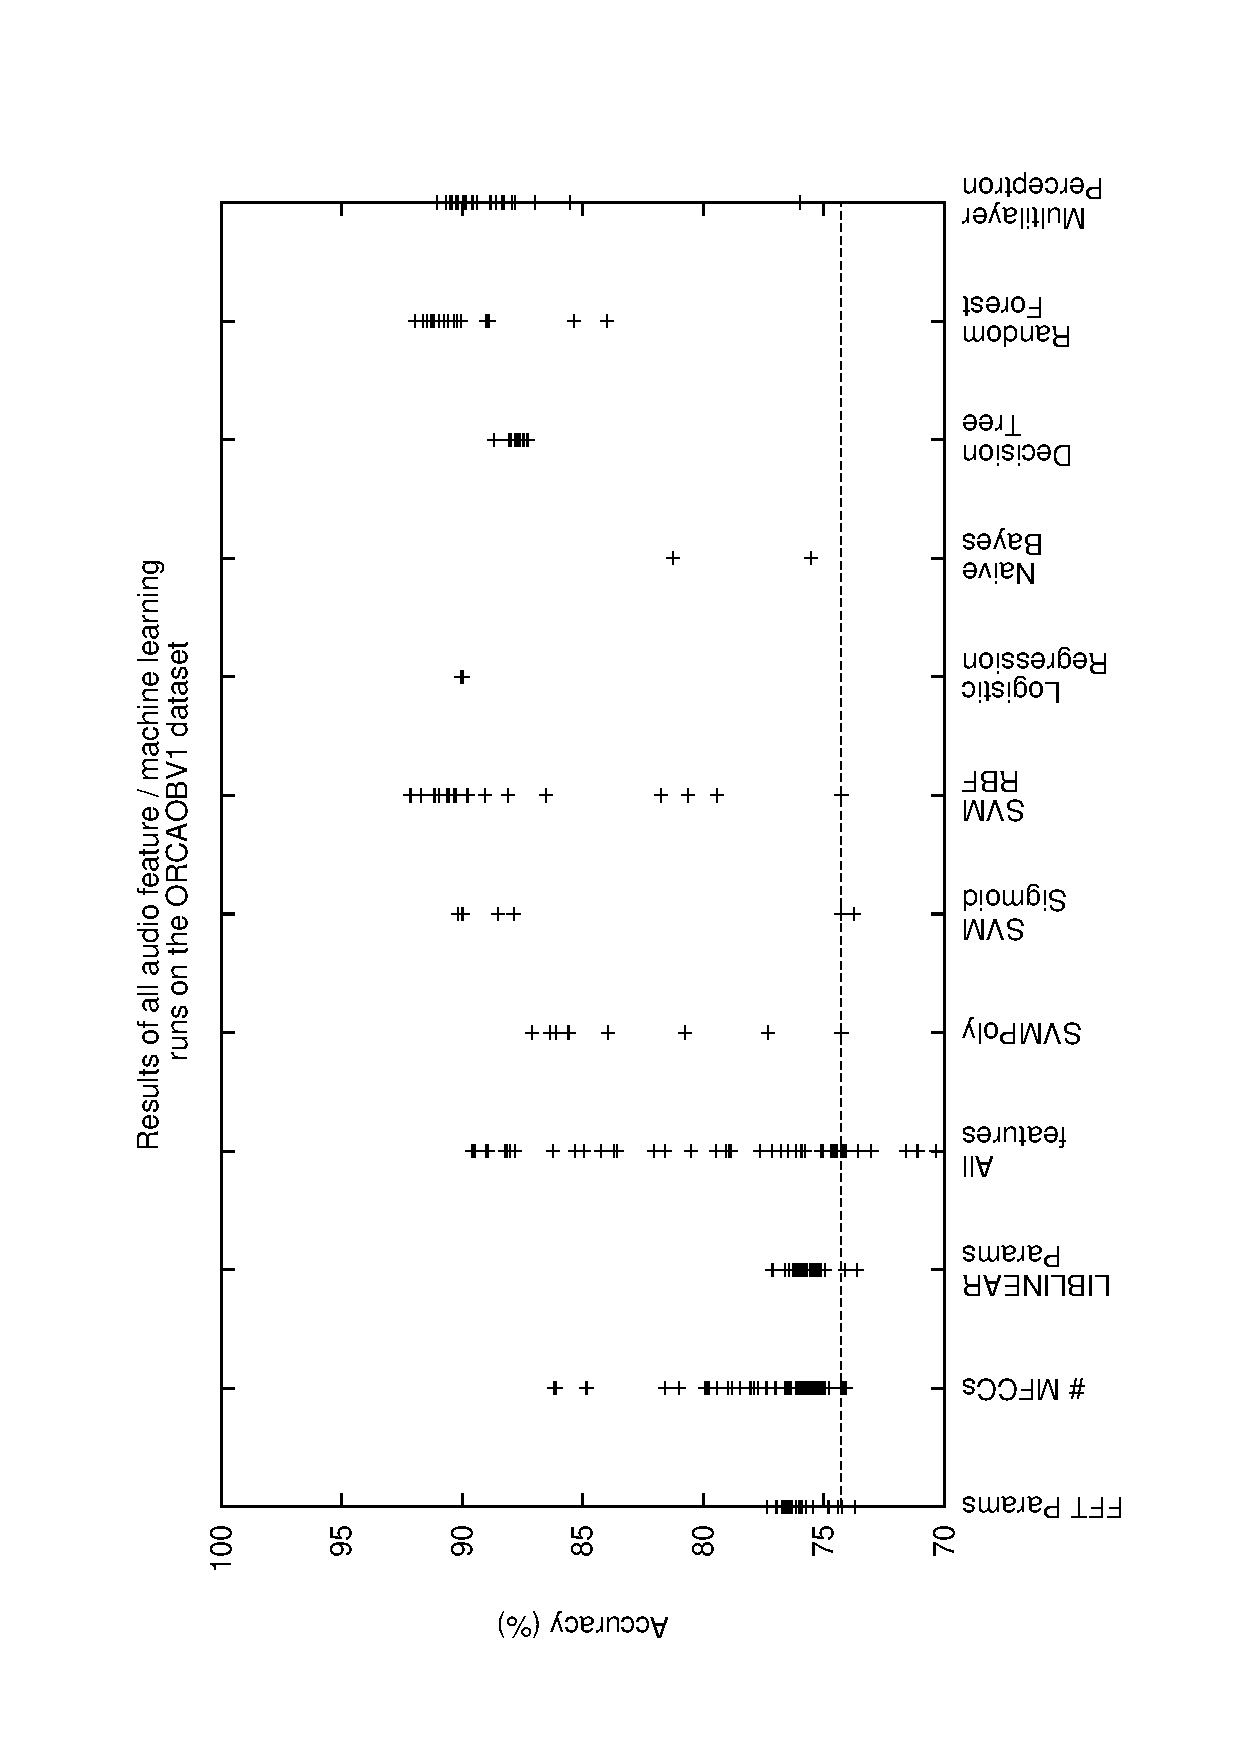
\includegraphics[width=\columnwidth]{figures/gnuplot-obv-all-data}
\caption{Shown are 831 data points from all the runs with different
  combinations of audio features and classifier and different
  parameter settings for each.}
\label{fig:gnuplot-obv-all-data}
\end{figure}

From these tables we can see that choosing an appropriate set of audio
feature extractors and machine learning algorithm can lead to good
classification performance.  When the various hyper-parameters of
these algorithms are optimized, even better performance can be
obtained.  When using only 13 MFCCs and an SVM with a linear kernel,
the maximum classification accuracy that was obtained was a poor
76.97\%, as can be seen in Table \ref{table:obv-fft}.  Increasing the
number of MFCC coefficients surprisingly greatly increased the
performance of the orca/background/voice classification task, and as
shown in Table \ref{table:obv-numMfccs} the highest classification
accuracy obtained was 86.17\%.  This is not usually a parameter that
needs to be adjusted when studying human speech or music, therefore this is a
surprising result.  As more features were added classification
performance increased in general.  This is a different result than was
obtained using a smaller dataset where the addition of Yin features
hurt performance \cite{ness2008chants}.  The maximum classification
accuracy was obtained using 70 MFCC coefficents and all possible audio
features.  For future work, it would be interesting to look at
including even more audio features, to see if the classification
accuracy continues to increase.

After finding the optimal audio features using an SVM with a linear
kernel, these features were used as input to a series of machine
learning classifiers.  The lowest performers were SVM with a
polynomial kernel (76.92\%), Naive Bayes (81.25\%).  The rest of the
learners performed well, with Decision Trees giving a maximum accuracy
of 88.67\%, Linear SVM of 89.53\%, Logistic Regression at 90.04\%, SVM
with a Sigmoid kernel of 90.18\%, Multilayer Perceptron at 91.04\%,
Random Forest with 91.97\%, and SVM with a Radial Basis Function
kernel at 92.12\%.  ALl the accuracy results in this chapter are
show in Figure \ref{fig:gnuplot-obv-all-data}.  In this figure, a
dashed line at 74.26\% represents the performance of the ZeroR
classifier.  From this graph we can see the SVM with an RBF kernel
performed the best, but that the Random Forest classifier was close
behind.  All the audio feature / classifier combinations showed
dramatic performance changes when parameters were changed, which
highlights the importance of doing parameter searches.

However, when doing actual classification experiments, it must be
decided if the rise in classification performance is offset by the
training and testing time.  For the LIBLINEAR classifier to obtain a
performance of 89.53\%, it took 18.3 minutes to train and predict the
ORCAOBV1 dataset.  For SVM with an RBF kernel it took 19.4 hours to do
the same thing, which means that it took almost a two-fold increase in
order of magnitude in time for a 2.59\% rise in performance.


\section{Scaling and Grid Computation}


The purpose of these experiments is to find the combination of audio
features and machine learning algorithm that gives the highest
performance for segmenting recordings into orca/background/voice, and
to then use this combination to predict classes for all recordings in
the Orchive.  In order to investigate the performance of the
classification of recordings into orca, background and voice, we
trained a SVM with a section of 30 and 240 seconds of hand trimmed
data.

These results were generated using the bextract/sfplugin combination
from \textit{Marsyas}, which are two different programs, the first of which
``bextract'' extracts audio features from a collection of audio files
and trains a machine learning classifier.  This trained classifier is
then used by the ``sfplugin'' program to extract audio features from
an audio source and to classify it.  The sfplugin program allows for
feature extraction and machine learning in a single executable, which
allows for a dramatic speedup because audio features do not need to be
written to disk and reread from disk.  In this hybrid program, audio
features train the machine learning system directly.

I first trained a model with bextract, and then used the sfplugin
program in \textit{Marsyas} to classify all the recordings in the Orchive on
the Hermes/Nestor cluster, part of the Westgrid computational
resource.  For this, I divided the data into sets of 1\%, 5\%, 10\%
and 100\% of the Orchive.  The timing results of these datasets run on
10 computers are shown in Table \ref{table:full-orchive-performance}.
From this, we can see that the classifier that had more data took
longer to classify, and that the speedup from taking samples of the
data was almost linear.


\begin{table}
\centering
\begin{tabular}{|c|c|c|} 
\hline
Training data & \% of Orchive & Run time \\
\hhline{|~|~|~|}
 (sec)        &               & (DD:HH:MM:SS) \\
\hhline{|=|=|=|}
30            &      1      &    00:00:05:18      	 \\
30            &      5      &    00:00:25:20         \\
30            &      10     &    00:00:50:58         \\
30            &      100    &    00:09:01:05         \\
\hline
240           &      1      &    00:06:16            \\
240           &      5      &    00:00:31:21         \\
240           &      10     &    00:04:47:12         \\
240           &      100    &    02:04:18:32         \\
\hline
\end{tabular}
\caption{Performance results of timing on subsets of the entire
  Orchive dataset using ten 2.66-GHz Intel Xeon x5650 cores.}
\label{table:full-orchive-performance}
\end{table}

%
% Downsampling
%
\section{Downsampling}

One way to reduce the total number of feature vectors, thereby
lowering feature size on disk and decreasing the training time and
testing time for machine learning classifiers is to downsample the
feature vectors at the time that features are calculated.  In this
case, downsampling is done by only outputting one feature vector each
$N$ times the feature is calculated.  In Table
\ref{table:obv-downsampling}, results are shown for using window sizes
from 512 to 4096 and downsampling rates from 1, where every feature
vector is output to 1000, where only every 1000th feature vector is
used.  What one would expect in this table is that a downsampling of 1
would give the highest accuracy, and greater amounts of downsampling
should either give the same accuracy until too few feature vectors are
used and performance would decrease.  In this table, the accuracy is
quite similar inside a single window size, for example, for the case
of a window size of 512, the difference in accuracies is 1.21\%.  This
tells us that in general, with the large amount of data that is in
this training set, any amount of downsampling will give approximately
the same results.  This could be used to great effectiveness when
expanding the set of the training data to a larger size than the
11,041 clips used in this section as is shown by the dramatic
reduction in training and test times that are seen in Table
\ref{table:obv-downsampling}.

\begin{table}
\begin{tabular}{|l|l|l|l|l|l|}
\hline
\multicolumn{3}{|c|}{FFT param} & \multicolumn{2}{c|}{Time (sec)} & Accuracy \\
\hhline{|-|-|-|-|-|~|}
ws & hp & downsampling & Train & Predict & \multicolumn{1}{c|}{(\%)} \\
\hhline{|=|=|=|=|=|=|}
512 & 256 & 1       &    31.27  &  2.06  &  75.90  \\
512 & 256 & 10      &     3.26  &  0.21  &  76.01  \\
512 & 256 & 100     &     0.31  &  0.03  &  75.82  \\
512 & 256 & 1000    &     0.07  &  0.02  &  75.00  \\
1024 & 512 & 1      &    17.80  &  1.05  &  75.76  \\
1024 & 512 & 10     &     1.64  &  0.12  &  75.76  \\
1024 & 512 & 100    &     0.15  &  0.02  &  76.52  \\
1024 & 512 & 1000   &     0.02  &  0.00  &  77.67  \\
\hline
2048 & 1024 & 1     &     8.60  &  0.52  &  75.92  \\
2048 & 1024 & 10    &     0.86  &  0.06  &  75.96  \\
2048 & 1024 & 100   &     0.08  &  0.01  &  74.90  \\
2048 & 1024 & 1000  &     0.01  &  0.00  &  73.08  \\
4096 & 2048 & 1     &     3.96  &  0.30  &  75.93  \\
4096 & 2048 & 10    &     0.36  &  0.04  &  75.89  \\
4096 & 2048 & 100   &     0.09  &  0.01  &  \textbf{76.54}  \\
4096 & 2048 & 1000  &     0.03  &  0.02  &  57.69  \\
\hline
\end{tabular}
\caption{Table showing the results of different amounts of
  downsampling on classification performance with the LIBLINEAR SVM
  using MFCC audio features.  Note that approximately 3x as
  much data points as this were calculated but were omitted due to
  space.  These omitted data points showed the same approximate
  performance as those shown here.}
\label{table:obv-downsampling}
\end{table}

For each of these machine learning methods, a confusion matrix was
obtained. This matrix shows the distribution of predictions and
mispredictions for each class. If the dataset had been perfectly
classified all the classifications would fall on the diagonal.  The
confusion matrix for one of the settings of the Random Forest is shown
in Table \ref{table:OBVConfusionMatrix}.  From this table, one can see
that in the majority of cases, the classifier predicted the label
correctly, but that in the case of background labels, there were a
large number of background labels that were predicted as orca calls at
a level of approximately 26\%.  The inverse of this, where orca calls
were misclassified as background was much lower, with a
misclassification rate of approximately 4\%.  For this task, the time
taken to build model was 1279 seconds and the time taken to test the
model on training data was 34 seconds on a 2.67-GHz Xeon x5550
processor.

\begin{table}
\begin{tabular}{|c|c|c|c|}
\hline
           & background & orca & voice \\
\hline
background & 79.4 &  20.5  &  0.1      \\
orca       & 3.7  &  96.1  &  0.1      \\
voice      & 1.0  &  13.3  &  85.7     \\
\hline
\end{tabular}
\caption{Confusion matrix for the Random Forest machine
  learning classifier.  The labels along the top represent the
  classifications by the machine learning classifier and those on the
  left side show the ground truth.  For a classifier that predicts
  each label perfectly, all the numbers would be on the diagonal. From
  this we can see that the majority of labels predicted classifier
  match the ground truth, but that the classifier mispredicts
  background labels as orca calls at a level of approximately 26\%.  }
\label{table:OBVConfusionMatrix}
\end{table}

However, in some cases, higher accuracies for larger downsampling
rates is seen.  Upon further investigation, this turned out to be due
to the fact that many clips were of short duration, with many being
approximately 0.2 seconds in length.  At this resolution, all of the
feature vectors for some of these short recordings were discarded, and
they did not become part of either the training or test set.  For this
reason, all subsequent tables do not use downsampling, and to
accommodate the long training and prediction times, a large cluster
was used, and each job was given the maximum allowable three-day run
time to complete.


\section{Call classification}

Once the large amount of data has been segmented into sections that
have been identified as orca calls, I am now interested in
classifying these call types based on the call catalog of Ford
\cite{ford1987catalogue}.  As an additional and related task, I am
also interested in classifying these call types based on the clan, pod,
subpod, matriline and individual that made the calls.  These are
overlapping tasks as some call types are only made by one pod, so
classifying some of them would automatically give the pod they came
from, like the N47 call.  Other call types are very distinct from pod to
pod, and can be handled as separate classification tasks, and others
are so similar, like N3, that it is difficult for an untrained person
to differentiate between call types made by different pods and would likely
be a difficult machine learning task.

I name the call catalog dataset used in this section ORCACALL1.  It
contains 2954 different clips containing orca calls as labelled by
people trained to do NRKW orca call classification.  The names,
numbers of instances in the ORCACALL1 dataset, and a few spectrograms
of representative exemplars are shown in Table
\ref{table:calls-table}.  It should be noted that the call types are
not present in equal abundance as a number of the call types are less
frequently vocalized by the orcas in the recordings that were
examined.  Some of the less frequently found call types are N08, N10,
N23 and N25.  Because of this inequal class distribution, a ZeroR
classifier would give a classification accuracy of 45\%; If the
classes had equal numbers of instances, the performance of the ZeroR
classifier would be 8.3\%.  For the work in this thesis, it was
determined that having a wider set of instances for training would be
preferable to the dramatic pruning that would have to occur if the
largest class (N04 : 1281 instances) would have to be pruned to the
size of the smallest (N08 : 22 instances).  Work is ongoing in the
creation of the ORCACALL2 dataset, which will have a wider set of call
types and more instances of all call types, with preference given to
less frequently produced call types.

The clips for this were obtained directly from the expert users, and
often contained small amounts of silence or boat noise before and
after the clip.  In addition, many of the clips contained very distant
orca calls, so distant that the calls were not clearly visible on the
spectrogram through the noise.  I concatentated all the clips
together, and generated a dataset where only the calls that were
visible in the spectrogram are represented, this gave a dataset of
1566 clips.  However, many of these clips were still quiet distant, so
I generated a second dataset of just the loud calls, which gave a
dataset of 658 calls.  These clips were run through the same
processing steps below as the untrimmed clips, and results are
presented alongside them.

\begin{table}
\begin{tabular}{|l|l|l|l|l|}
\hline
Call     &  \# Calls  & \# Trimmed & \# Trimmed         &  Representative  \\
type     &            & calls      & loud calls         &    spectrogram    \\
\hline
 N01     &  364       &  296  &   85                &   \includegraphics[height=1.5cm] {figures/catalog/A36-N01-062802-D004-12218.png} \\ \hline
 N02     &  123       &   95  &   53                &   \includegraphics[height=1.5cm] {figures/catalog/A36-N02-063002-D005-10750.png} \\ \hline
 N03     &  244       &  106  &   56                &   \includegraphics[height=1.5cm] {figures/catalog/A36-N03-071506-D017-10139.png} \\ \hline
 N04     &  1281      &  281  &   64                &   \includegraphics[height=1.5cm]  {figures/catalog/A36-N04-063002-D005-10843.png} \\ \hline
 N05     &  157       &  142  &   74                &   \includegraphics[height=1.5cm] {figures/catalog/A35-N05-070606-D011-04146.png} \\ \hline
\end{tabular}
\caption{Part 1 of table of call types in the ORCACALL1 dataset.  All call types were
  annotated by users trained in recognizing orca vocalizations.  Some
  call types, such as N04 are more frequently vocalized by orcas, and are
  present in higher abundance in this dataset.  Work is ongoing in
  creating the ORCACALL2 dataset, which will have a larger set of
  call types.}
\label{table:calls-table}
\end{table}

\begin{table}
\begin{tabular}{|l|l|l|l|l|}
\hline
Call     &  \# Calls  & \# Trimmed & \# Trimmed         &  Representative  \\
type     &            & calls      & loud calls         &  spectrogram    \\
\hline
 N07     &   108      &             91  &   59                    &  \includegraphics[height=1.5cm] {figures/catalog/A08-N07-071110-D013-01151.png} \\ \hline
 N08     &   22       &             10  &    5                    &  \includegraphics[height=1.5cm] {figures/catalog/A04-N08-071906-D020-13145.png} \\ \hline
 N09     &   413      &            328  &  129                    &  \includegraphics[height=1.5cm] {figures/catalog/A12-N09-070102-D005-14103.png} \\ \hline
 N10     &   39       &             26  &   19                    &  \includegraphics[height=1.5cm] {figures/catalog/A36-N10-063002-D005-10954.png} \\ \hline
 N23     &   30       &             18  &    9                    &  \includegraphics[height=1.5cm] {figures/catalog/I31-N23-070706-D011-10950.png} \\ \hline
 N25     &   27       &             12  &    6                    &  \includegraphics[height=1.5cm] {figures/catalog/I15-N25-081206-D044-02059.png} \\ \hline
 N47     &   177      &            161  &   99                    &  \includegraphics[height=1.5cm] {figures/catalog/A12-N47-080210-D056-15012.png} \\ \hline
\end{tabular}
\caption{Part 2 of table of call types in the ORCACALL1 dataset.}
\label{table:calls-table}
\end{table}

It should be noted though that there are other forms of information
that can be used by scientists in the future when using classifiers
from this work, the most important being direct visual observation
combined with the use of the photo identification catalog.  This could
be combined with acoustic arrays of hydrophones to localize individual
whales.

In this section, I will follow a similar strategy to that for the
classification task above and will discuss the similarities and
differences when classifying call types as opposed to simply classifying
audio into orca/background/voice as in the ORCAOBV1 dataset.  The
dataset with call types will be referred to as ORCACALL1 in the following
tables.

In order to classify the clips in the ORCACALL1 dataset, I use a
different experimental procedure to that used in the ORCAOBV1 results
presented in the previous section.  Each clip was considered to have
been presegmented by either the user or the machine learning system
and results on a per clip-level were generated.  These clip level
decisions were made using a voting metaphor, where each feature vector
in a clip was assigned a label by the classifier individually, and the
clip was labeled with the label that occurred the most often.

%
% FFT Parameters
%
\subsection{FFT Parameters}

Following a similar procedure to that carried out for ORCAOBV1
dataset, a parameter scan of different window sizes, hop sizes and
texture window sizes was performed, with results shown in Table
\ref{table:calls-fft}.  In this table, there is a larger variation in
accuracy than was seen in the case of the ORCAOBV1 dataset and the
highest accuracy that was obtained was 56\%, which was obtained with a
window size of 4096 and a memory size of 10 for the trimmed loud
clips.  However, the results for a window size of 2048 and a memory
size of 10 gave almost the same results of 55\% but with half as long
an integration time, thus allowing for shorter integration
times. Because of this, for subsequent tables, a window size of 2048,
hop size of 1024 and memory size of 10 was used to facilitate
comparison with the results for the ORCAOBV1 dataset.  It is
interesting to note that the trimmed clips did approximately as well
as the untrimmed clips, however the trimmed loud clips had higher
accuracy.  This can be explained by the fact that MFCC features are
cepstrums, which are spectrums of spectrums, and for clips with a
larger signal in them, the feature vectors obtained would be more
distinct from noise vectors for loud clips than for quiet clips.

\begin{table}
\begin{tabular}{|c|c|c|c|c|c|c|c|}
\hline
\multicolumn{3}{|c|}{FFT param} & \multicolumn{2}{c|}{Time (sec)} & \multicolumn{3}{c|}{\% Accuracy} \\
\hhline{|-|-|-|-|-|-|-|-|}
ws & hp & mem & Extract & Train & All & Trimmed & Trimmed Loud \\
\hhline{|=|=|=|=|=|=|=|=|}
512  & 256  & 1    &    141.79  &    87.32  &  47  & 39 & 48 \\
512  & 256  & 2    &    127.92  &   505.95  &  47  & 44 & 50 \\
512  & 256  & 5    &    153.62  &   314.00  &  48  & 46 & 50 \\
512  & 256  & 10   &    140.79  &   339.46  &  48  & 45 & 50 \\
512  & 256  & 20   &    118.44  &   368.40  &  49  & 48 & 50 \\
\hline
1024 & 512  & 1    &     90.56  &    30.82  &  44  & 39 & 44 \\
1024 & 512  & 2    &    117.79  &   177.41  &  48  & 44 & 47 \\
1024 & 512  & 5    &    108.07  &   178.74  &  48  & 45 & 52 \\
1024 & 512  & 10   &    102.28  &   137.23  &  50  & 48 & 53 \\
1024 & 512  & 20   &     92.13  &   151.60  &  51  & 49 & 55 \\
\hline
2048 & 1024 & 1    &     86.24  &    13.75  &  44  & 43 & 47 \\
2048 & 1024 & 2    &     83.15  &   118.59  &  49  & 48 & 47 \\
2048 & 1024 & 5    &     72.37  &    69.04  &  49  & 51 & 52 \\
2048 & 1024 & 10   &     85.48  &    62.31  &  52  & 48 & 55 \\
2048 & 1024 & 20   &     78.48  &    85.45  &  52  & 48 & 55 \\
\hline
4096 & 2048 & 1    &     76.07  &     5.34  &  46  & 46 & 47 \\
4096 & 2048 & 2    &     83.15  &    38.11  &  49  & 47 & 48 \\
4096 & 2048 & 5    &     72.37  &    30.38  &  51  & 50 & \textbf{56} \\
4096 & 2048 & 10   &     75.06  &    28.24  &  52  & 47 & 53\\
4096 & 2048 & 20   &     77.32  &    27.35  &  52  & 48 & 55 \\
\hline
\end{tabular}
\caption{Table of MFCC results with different window
  sizes using the LIBLINEAR classifier.  In this and subsequent
  tables, ``ws'' refers to the size of the FFT window in samples,
  ``hp'' refers the hop size between sequent FFT frames in samples,
  and ``mem'' refers to the size of the texture window in frames.
  Longer texture window sizes have been omitted as they showed
  anomalous behaviour due to the short size of the clips as compared
  to the long integration time.}
\label{table:calls-fft}
\end{table}

%
% Different numbers of MFCCs
%
\subsection{Number of MFCC coefficients}

As in the ORCAOBV1 dataset, a parameter scan of the number of MFCC
components was carried out, with results shown in Table
\ref{table:calls-numMfccs}.  The highest performance obtained was for
a window size of 4096 and 100 MFCCs with an accuracy of 58\%, with a
window size of 2048 and 100 MFCCs yielding an accuracy of 54\%.  These
results show a similar trend to the results obtained for ORCAOBV1 with
more MFCCs giving better results.  Using a window size of 4096 samples
with a hop size of 2048 samples at 44100 samples/sec gives an
integration time of 46.4 milliseconds, and 10 of these windows (given
a memory size of 10 frames) would result in a total time of 464
milliseconds or almost half a second.  Using a window size of 2048
would give a total time of half that or 232 milliseconds.  Like in
Table \ref{table:calls-fft} the performance of classifiers with loud
trimmed clips did significantly better than for untrimmed and the
whole set of trimmed clips.  This is likely due to the fact that for
clips with greater signal, MFCC features produce feature vectors that
are more distinct from clips with less signal, or clips of boat noise.

\begin{table}
%% \begin{tabular}{|l|l|l|l|l|l|}
%% \hline
%% \multicolumn{3}{|c}{FFT param} & \multicolumn{1}{|c|}{Time (sec)} & Accuracy \\
%% \hhline{|-|-|-|-|~|}
%% ws & hp & Num MFCCs & Train & \multicolumn{1}{c|}{(\%)} \\
%% \hhline{|=|=|=|=|=|}
\begin{tabular}{|c|c|c|c|c|c|c|c}
\hline
\multicolumn{3}{|c|}{FFT param} & \multicolumn{1}{c|}{Time (sec)} & \multicolumn{3}{c|}{\% Accuracy} \\
\hhline{|-|-|-|-|-|-|-|-|}
ws & hp & mem & Train & All & Trimmed & Trimmed Loud \\
\hhline{|=|=|=|=|=|=|=|=|}
512 & 256 & 1      &        30.86  &    43   &  21  &  21 \\
512 & 256 & 5      &       125.01  &    43   &  36  &  41 \\
512 & 256 & 10     &       217.63  &    48   &  46  &  50 \\
512 & 256 & 15     &       325.26  &    49   &  47  &  53 \\
512 & 256 & 25     &       675.81  &    51   &  54  &  58 \\
512 & 256 & 30     &      1059.44  &    51   &  53  &  59 \\
512 & 256 & 40     &      1153.37  &    51   &  54  &  61 \\
\hline
1024 & 512 & 1     &        15.20  &    43  &  21  &  21 \\
1024 & 512 & 5     &        50.34  &    43  &  36  &  41 \\
1024 & 512 & 10    &       122.80  &    49  &  46  &  50 \\
1024 & 512 & 15    &       155.82  &    50  &  49  &  55 \\
1024 & 512 & 25    &       336.11  &    52  &  55  &  56 \\
1024 & 512 & 50    &       836.08  &    53  &  58  &  58 \\
1024 & 512 & 70    &      1850.25  &    53  &  57  &  56 \\
1024 & 512 & 100   &      2667.66  &    53  &  60  &  62 \\
\hline
2048 & 1024 & 1    &         5.24  &    43 &  21  &  21 \\
2048 & 1024 & 5    &        22.52  &    44 &  35  &  38 \\
2048 & 1024 & 10   &        50.33  &    49 &  46  &  52 \\
2048 & 1024 & 15   &        75.94  &    51 &  51  &  56 \\
2048 & 1024 & 25   &       192.55  &    53 &  58  &  56 \\
2048 & 1024 & 50   &       524.04  &    54 &  60  &  62 \\
2048 & 1024 & 70   &       887.34  &    54 &  60  &  62 \\
2048 & 1024 & 100  &      1474.60  &    54 &  59  &  62 \\
\hline
4096 & 2048 & 1    &         2.51  &    43 &  20  &  21 \\
4096 & 2048 & 5    &         9.18  &    44 &  31  &  38 \\
4096 & 2048 & 10   &        21.19  &    50 &  41  &  50 \\
4096 & 2048 & 15   &        34.65  &    54 &  48  &  50 \\
4096 & 2048 & 25   &        78.55  &    57 &  57  &  56 \\
4096 & 2048 & 50   &       213.46  &    58 &  57  &  \textbf{67} \\
4096 & 2048 & 70   &       346.59  &    58 &  57  &  \textbf{67} \\
4096 & 2048 & 100  &       668.68  &    58 &  56  &  65 \\
\hline
\end{tabular}
\caption{Table of MFCC results with different numbers of MFCC
  coefficients using the LIBLINEAR classifier and the ORCACALL1 dataset}
\label{table:calls-numMfccs}
\end{table}

%
% LIBLINEAR parameters
%
\subsection{LIBLINEAR parameters}

A parameter sweep of using different solvers and values of C for
LIBLINEAR was then carried out, with results shown in Table
\ref{table:calls-liblinear}.  In this table, several experimental
conditions gave the same performance of 55\%.  However, unlike in the
ORCAOBV1 case, there was considerably more variation in performance
with this classifier.  In terms of speed, the L2-regularized L2-loss
support vector classification (primal) gave the fastest consistent
performance as can be seen in Figure
\ref{fig:gnuplot-calls-liblinear-time}.  What is interesting here is
that even though the different values of C do not cause big
differences in classification accuracy, depending on the solver, they
can a have dramatic impact on the time it takes to reach a solution.
For this dataset, it appears that the best solver with the most
consistent performance is the L2-regularized L2-loss support vector
classification (primal).  In these experiments, again the set of
trimmed loud clips performed better, which is expected for clips with
a greater signal in them with MFCC features.

\begin{figure}[t]
\centering
\includegraphics[width=\columnwidth]{figures/gnuplot-calls-liblinear-time}
\caption{The amount of time that different solvers took to train a SVM
  model in LIBLINEAR.}
\label{fig:gnuplot-calls-liblinear-time}
\end{figure}


\begin{table}
%% \begin{tabular}{|l|l|l|l|}
%% \hline
%% \multicolumn{2}{|c}{LIBLINEAR param} & \multicolumn{1}{|c|}{Time (sec)} &  Accuracy \\
%% \hhline{|-|-|-|~|}
%% Solver & C & Train & \multicolumn{1}{c|}{(\%)} \\
%% \hhline{|=|=|=|=|}
\begin{tabular}{|c|c|c|c|c|c|}
\hline
\multicolumn{2}{|c|}{LIBLINEAR param} & \multicolumn{1}{c|}{Time (sec)} & \multicolumn{3}{c|}{\% Accuracy} \\
\hhline{|-|-|-|-|-|-|}
Solver & C & Train & All & Trimmed & Trimmed Loud \\
\hhline{|=|=|=|=|=|=|}
1 & 0.001   &       3.71  &    51  &  43  &  50 \\
1 & 1.0     &      31.16  &    53  &  45  &  50 \\
1 & 100.0   &     405.72  &    43  &  42  &  33 \\
2 & 0.001   &       3.55  &    51  &  44  &  50 \\
2 & 1.0     &       3.73  &    53  &  45  &  50 \\
2 & 1000.0  &       3.78  &    53  &  45  &  50 \\
\hline
3 & 0.001   &       3.40  &    51  &  50  &  \textbf{55} \\
3 & 1.0     &      18.84  &    54  &  52  &  53 \\
3 & 1000.0  &     425.39  &    33  &  35  &  50 \\
4 & 0.001   &       2.28  &    49  &  47  &  \textbf{55} \\
4 & 1.0     &      32.90  &    52  &  49  &  \textbf{55} \\
4 & 1000.0  &    9557.33  &    46  &  48  &  \textbf{55} \\
\hline
5 & 0.001   &      15.43  &    47   &  43  &  53 \\
5 & 1.0     &      34.04  &    53   &  45  &  50 \\
5 & 1000.0  &      31.91  &    53   &  45  &  50 \\
6 & 0.001   &       5.52  &    43   &  39  &  41 \\
6 & 1.0     &      14.32  &    54   &  46  &  52 \\
6 & 1000.0  &      17.12  &    54   &  45  &  53 \\
7 & 0.001   &       5.20  &    45   &  41  &  41 \\
7 & 1.0     &      12.45  &    54   &  48  &  53 \\
7 & 1000.0  &     635.40  &    50   &  48  &  53 \\
\hline
\end{tabular}
\caption{A table showing the results with the ORCACALL1 dataset of
  doing a parameter search over a wide number of values of C and using
  the different solvers in the LIBLINEAR package.}
\label{table:calls-liblinear}
\end{table}

%
% MIR Features
%
\subsection{MIR Features}

In order to investigate the manner in which different audio features
affect classification performance, a series of experiments was carried
out in which different audio features and combinations of these audio
features was used, with a similar methodology to that used on the
ORCAOBV1 dataset.

%% In the first test, different window and hop sizes were used as input
%% to the MFCC algorithm, with a texture memory size set at 10.  These
%% results are shown in Table \ref{table:calls-different-mfcc}.  Unlike
%% in the ORCAOBV1 case, the best classification accuracy was obtained
%% for longer window sizes, with the best performance being at a window
%% size of 4096, which gave a classification accuracy of 53\%.

%% \begin{table}
%% %% \begin{tabular}{|l|l|l|l|l|}
%% %% \hline
%% %% \multicolumn{2}{|c|}{FFT param} & \multicolumn{2}{c|}{Time (sec)} & Accuracy \\
%% %% \hhline{|-|-|-|-|~|}
%% %% ws & hp & Extract & Train &  \multicolumn{1}{c|}{(\%)} \\
%% %% \hhline{|=|=|=|=|=|}
%% \begin{tabular}{|c|c|c|c|c|c|c|c|}
%% \hline
%% \multicolumn{3}{|c|}{FFT param} & \multicolumn{2}{c|}{Time (sec)} & \multicolumn{3}{c|}{\% Accuracy} \\
%% \hhline{|-|-|-|-|-|-|-|-|}
%% ws & hp &  Extract & Train & All & Trimmed & Trimmed Loud \\
%% \hhline{|=|=|=|=|=|=|=|=|}
%% 256 & 128 &    228.01  &   70.64  &    47  \\
%% 512 & 256 &    176.47  &   28.56  &    48  \\
%% 1024 & 512 &   131.70  &   15.56  &    49  \\
%% 2048 & 1024 &  102.47  &    7.60  &    51  \\
%% 4096 & 2048 &   98.47  &    3.62  &    53  \\
%% \hline
%% \end{tabular}
%% \caption{Table showing the classification accuracy and timing when
%%   using different FFT window sizes on MFCC features using a linear SVM
%%   kernel using the ORCACALL1 dataset.}
%% \label{table:calls-different-mfcc}
%% \end{table}

When the RMS feature alone was used, a dramatic drop in performance
was seen, with the accuracy in each window size being 43\% as is seen
in Table \ref{table:calls-different-rms}.  This is an expected
behaviour because with the ORCACALL1 database the loudness of
different call types is uncorrelated with the call type and is
dependent instead on the distance of the orca from the hydrophone.  It
is also interesting that for the trimmed calls and trimmed loud calls
that the accuracy was very low, this is likely because the untrimmed
clips were actually being classified due to the amount of noise in
them, not in their actual performance on classifying different calls.
It is very interesting that for RMS features, the trimmed and trimmed
loud clips performed much more poorly than the untrimmed calls.  This
is likely due to the classification algorithm actually classifying the
untrimmed clips based on the amount of noise in them, rather than on
the actual signal in them.  Given the nature of the RMS feature, that
it basically is a measure of the loudness of a clip, this is a likely
outcome, and shows us that on their own, RMS features are not a good
way to classify calls.

\begin{table}
%% \begin{tabular}{|l|l|l|l|l|}
%% \hline
%% \multicolumn{2}{|c|}{FFT param} & \multicolumn{2}{c|}{Time (sec)} & Accuracy \\
%% \hhline{|-|-|-|-|~|}
%% ws & hp & Extract & Train &  \multicolumn{1}{c|}{(\%)} \\
%% \hhline{|=|=|=|=|=|}
\begin{tabular}{|c|c|c|c|c|c|c|}
\hline
\multicolumn{2}{|c|}{FFT param} & \multicolumn{2}{c|}{Time (sec)} & \multicolumn{3}{c|}{\% Accuracy} \\
\hhline{|-|-|-|-|-|-|-|}
ws & hp & Extract & Train & All & Trimmed & Trimmed Loud \\
\hhline{|=|=|=|=|=|=|=|}
256 & 128        &   178.01  &    7.00  &    \textbf{43}  & 17 & 20 \\
512 & 256        &   135.04  &    3.41  &    \textbf{43}  & 23 & 20 \\
1024 & 512       &   100.13  &    1.66  &    \textbf{43}  & 22 & 20 \\
2048 & 1024      &    88.20  &    0.82  &    \textbf{43}  & 22 & 20  \\
4096 & 2048      &    86.54  &    0.33  &    \textbf{43}  & 22 & 20 \\
\hline
\end{tabular}
\caption{Table using audio from the ORCACALL1 dataset showing the
  effect of window size on classification performance with LIBLINEAR
  using the Root Mean Square (RMS) energy of a signal as a feature.}
\label{table:calls-different-rms}
\end{table}

Surprisingly, the use of statistical measures of the spectrum, as
shown in Table \ref{table:calls-different-spectral}, gave poor
classification accuracy, with a maximum classification accuracy of
43\%.  This is likely because the broad spectral characteristics of
these measures did not accurately capture important factors about the
differences between calls.  Another confounding factor is the
directionality of calls which means that the orientation of the
vocalizing orca to the receiving hydrophone is a confounding variable
here \cite{miller2002mixed}.  The results for trimmed and untrimmed
calls are also low, as was seen for RMS, which is likely because in
the case of untrimmed clips, the classifier was actually classifying
the clips by the spectral characteristics of the noise in the
untrimmed clips, and not classifying the actual calls.  Like in the
case of RMS features, the trimmed and untrimmed clips perform
significantly worse than untrimmed clips, but in this case instead of
the loudness of a clip, the classifier was likely taking advantage of
the spectral characteristics of noise in the untrimmed clips.

\begin{table}
%% \begin{tabular}{|l|l|l|l|l|l|}
%% \hline
%% \multicolumn{1}{|c|}{Feature} &\multicolumn{2}{c|}{FFT param} & \multicolumn{2}{c|}{Time (sec)} & Accuracy \\
%% \hhline{|~|-|-|-|-|~|}
%% Extractor & ws & hp & Extract & Train  &  \multicolumn{1}{c|}{(\%)} \\
%% \hhline{|=|=|=|=|=|=|}
\begin{tabular}{|c|c|c|c|c|c|c|c|}
\hline
\multicolumn{3}{|c|}{FFT param} & \multicolumn{2}{c|}{Time (sec)} & \multicolumn{3}{c|}{\% Accuracy} \\
\hhline{|-|-|-|-|-|-|-|-|}
ws & hp & mem & Extract & Train & All & Trimmed & Trimmed Loud \\
\hhline{|=|=|=|=|=|=|=|=|}
centroid & 256 & 128       &   215.26  &    6.99  &  \textbf{43}  & 26 & 20 \\
centroid & 512 & 256       &   144.23  &    3.10  &  \textbf{43}  & 26 & 20 \\
centroid & 1024 & 512      &   119.32  &    1.58  &  \textbf{43}  & 25 & 20 \\
centroid & 2048 & 1024     &   102.19  &    0.85  &  \textbf{43}  & 25 & 20 \\
centroid & 4096 & 2048     &    96.78  &    0.32  &  \textbf{43}  & 22 & 18 \\
\hline
flux & 256 & 128           &   218.31  &    7.43  &  \textbf{43}  & 21 & 20 \\
flux & 512 & 256           &   145.60  &    3.49  &  \textbf{43}  & 12 & 20 \\
flux & 1024 & 512          &   130.55  &    1.69  &  \textbf{43}  & 21 & 20 \\
flux & 2048 & 1024         &   107.72  &    0.91  &  \textbf{43}  & 21 & 20 \\
flux & 4096 & 2048         &    95.93  &    0.39  &  \textbf{43}  & 21 & 20 \\
\hline
rolloff & 256 & 128        &   205.94  &    6.08  &  \textbf{43}  & 31 & 17 \\
rolloff & 512 & 256        &   151.70  &    6.37  &  \textbf{43}  & 25 & 17 \\
rolloff & 1024 & 512       &   117.73  &    1.42  &  \textbf{43}  & 31 & 20 \\
rolloff & 2048 & 1024      &   109.10  &    0.71  &  \textbf{43}  & 31 & 20 \\
rolloff & 4096 & 2048      &    96.30  &    0.30  &  \textbf{43}  & 32 & 18 \\
\hline
kurtosis & 256 & 128       &   212.50  &    7.14  &  42           & 22 & 23 \\
kurtosis & 512 & 256       &   145.55  &    3.30  &  42           & 20 & 20 \\
kurtosis & 1024 & 512      &   123.56  &    1.91  &  \textbf{43}  & 22 & 23 \\
kurtosis & 2048 & 1024     &   108.91  &    0.74  &  42           & 23 & 21 \\
kurtosis & 4096 & 2048     &    95.63  &    0.39  &  42           & 23 & 21 \\
\hline
skewness & 256 & 128       &   232.54  &    7.31  &  \textbf{43}  & 23 & 20  \\
skewness & 512 & 256       &   179.31  &    3.51  &  \textbf{43}  & 25 & 23 \\
skewness & 1024 & 512      &   202.36  &    1.79  &  \textbf{43}  & 18 & 20 \\
skewness & 2048 & 1024     &   317.77  &    0.66  &  42           & 24 & 20 \\
skewness & 4096 & 2048     &   571.55  &    0.38  &  \textbf{43}  & 25 & 21 \\
\hline
\end{tabular}
\caption{Table showing the effect of using
  combinations of different statistical measures of the spectrum of a
  signal on classification performance with LIBLINEAR.}
\label{table:calls-different-spectral}
\end{table}

However, when using a combination of Chroma, SFM and SCF as shown in
Table \ref{table:calls-different-chroma}, a classification accuracy of
62\% was obtained, which was higher than using MFCCs alone, but unlike
the case for ORCAOBV1, this higher classification accuracy was not
universally seen, but was only observed in one experimental condition.
The highest classification accuracy obtained was for the trimmed clips
with chroma, SCF and SFM features.  This is unlike what was seen in
the previous two tables, and is likely due to the fact that a
combination of all these three features are actually classifying the
calls based on the content of the call, and not on the properties of
noise within the call.  This also means that these three features in
combination are likely good features to use for classifying calls.

\begin{table}
%% \begin{tabular}{|l|l|l|l|l|l|}
%% \hline
%% \multicolumn{1}{|c|}{Feature} &\multicolumn{2}{c|}{FFT param} & \multicolumn{2}{c|}{Time (sec)} & Accuracy \\
%% \hhline{|~|-|-|-|-|~|}
%% Extractor & ws & hp & Extract & Train & \multicolumn{1}{c|}{(\%)} \\
%% \hhline{|=|=|=|=|=|=|}
\begin{tabular}{|c|c|c|c|c|c|c|c|}
\hline
\multicolumn{3}{|c|}{FFT param} & \multicolumn{2}{c|}{Time (sec)} & \multicolumn{3}{c|}{\% Accuracy} \\
\hhline{|-|-|-|-|-|-|-|-|}
ws & hp & mem & Extract & Train & All & Trimmed & Trimmed Loud \\
\hhline{|=|=|=|=|=|=|=|=|}
chroma & 256 & 128    &   271.09  &   62.35  &  43  & 21 & 20 \\
chroma & 512 & 256    &   188.57  &   28.86  &  43  & 24 & 23 \\
chroma & 1024 & 512   &   134.10  &   14.60  &  43  & 20 & 24 \\
chroma & 2048 & 1024  &   107.68  &    7.53  &  43  & 25 & 27 \\
chroma & 4096 & 2048  &    89.70  &    4.42  &  43  & 27 & 30 \\
\hline
scf & 256 & 128       &   286.35  &  148.22  &  43  & 46 & 53 \\
scf & 512 & 256       &   192.18  &   70.59  &  43  & 36 & 48 \\
scf & 1024 & 512      &   131.62  &   35.30  &  43  & 46 & 47 \\
scf & 2048 & 1024     &   107.43  &   17.67  &  45  & 50 & 58 \\
scf & 4096 & 2048     &    99.94  &   11.43  &  51  & 55 & 47 \\
\hline
sfm & 256 & 128       &   311.21  &  167.47  &  43  & 35 & 48 \\
sfm & 512 & 256       &   203.01  &   71.52  &  43  & 42 & 48 \\
sfm & 1024 & 512      &   152.44  &   30.12  &  46  & 43 & 50 \\
sfm & 2048 & 1024     &   114.02  &   16.99  &  47  & 45 & 58 \\
sfm & 4096 & 2048     &   100.68  &    8.82  &  52  & 47 & 53 \\
\hline
all & 512 & 256       &   321.27  &  308.60  &  45  & 41 & 52 \\
all & 1024 & 512      &   218.39  &  163.69  &  48  & 45 & 53 \\
all & 2048 & 1024     &   147.61  &   74.98  &  53  & 52 & 59 \\
all & 4096 & 2048     &   124.08  &   39.91  &  59  & \textbf{62} & 52 \\
\hline
\end{tabular}
\caption{Table showing the classification performance
  of LIBLINEAR with different combinations of Chroma, Spectral Crest
  Factor (SCF) and Spectral Flatness Measure (SFM).}
\label{table:calls-different-chroma}
\end{table}

When using the YIN pitch determination algorithm, as is shown in Table
\ref{table:calls-different-yin} results were poor, with a maximum
accuracy of 43\%.  This is a surprising result, as one would hope that
the YIN algorithm would capture the pitch contour of the call and
would, therefore, lead to good classification.  Upon examination of
the data with the orchive v2.0 interface, the cause of this appeared
to be because the low signal/noise ratio (SNR) of the call preventing
the YIN algorithm from finding the correct pitch.  If better pitch
estimation could be carried out, the classification accuracy would
likely be higher when using this feature.  Again as in the case of RMS
and spectral features, the trimmed and trimmed loud calls perform
worse than the untrimmed calls, which likely means that the
classification algorithms were not classifying the clips in the
untrimmed case by the properties of their signal, but of the output of
the YIN algorithm on non orca call parts of the clips.

\begin{table}
%% \begin{tabular}{|l|l|l|l|}
%% \hline
%% \multicolumn{2}{|c|}{FFT param} & \multicolumn{1}{c|}{Time (sec)} & Accuracy \\
%% \hhline{|-|-|-|~|}
%% ws & hp & Train & \multicolumn{1}{c|}{(\%)} \\
%% \hhline{|=|=|=|=|}
\begin{tabular}{|c|c|c|c|c|c|}
\hline
\multicolumn{2}{|c|}{FFT param} & \multicolumn{1}{c|}{Time (sec)} & \multicolumn{3}{c|}{\% Accuracy} \\
\hhline{|-|-|-|-|-|-|}
ws & hp & Train & All & Trimmed & Trimmed Loud \\
\hhline{|=|=|=|=|=|=|}
256 & 128      &   181.64  &   \textbf{43} & 21 & 20 \\
512 & 256      &   166.88  &   \textbf{43} & 21 & 20 \\
1024 & 512     &   213.81  &   \textbf{43} & 21 & 20 \\
2048 & 1024    &   337.15  &   42          & 20 & 20 \\
4096 & 2048    &   560.11  &   \textbf{43} & 21 & 20 \\
\hline
\end{tabular}
\caption{Table showing the result of using the YIN pitch estimator as
  a feature for input to the LIBLINEAR SVM classifier with different
  window sizes and hop sizes.}
\label{table:calls-different-yin}
\end{table}

When all these audio features were combined, however, a large increase
in performance to a maximum of 71\% was achieved as can be seen in
Table \ref{table:calls-different-all}.  This value was seen in three
separate experimental conditions, and unlike in the case of ORCAOBV1
where chroma+SFM+SCF features alone gave approximately the same
classification accuracy as all features, in the ORCACALL1 dataset,
using all the features was considerably better than using just the
chroma+SFM+SCF features.  This is likely due to the increased
complexity of the classification task when doing call classification
and that the extra features captured different information about the
call.  In this set of experimental conditions, unlike the previous
ones, higher results were obtained with using the trimmed and trimmed
loud calls, which means that when using this larger set of features,
the classification is likely taking into account more of the actual
features of the calls, rather than on just classifying the calls based
on the spectral characteristics of the noise in the clips.

\begin{table}
%% \begin{tabular}{|l|l|l|l|l|}
%% \hline
%% \multicolumn{1}{|c|}{Feature} &\multicolumn{2}{c|}{FFT param} & \multicolumn{1}{c|}{Time (sec)} & Accuracy \\
%% \hhline{|~|-|-|-|~|}
%% Extractor & ws & hp & Train &  \multicolumn{1}{c|}{(\%)} \\
%% \hhline{|=|=|=|=|=|}
\begin{tabular}{|c|c|c|c|c|c|c|}
\hline
\multicolumn{3}{|c|}{FFT param} & \multicolumn{1}{c|}{Time (sec)} & \multicolumn{3}{c|}{\% Accuracy} \\
\hhline{|-|-|-|-|-|-|-|}
ws & hp & mem & Train & All & Trimmed & Trimmed Loud \\
\hhline{|=|=|=|=|=|=|=|}
spectral sfm scf & 512 & 256         &   399.36  &    54 & 54 & 62 \\
spectral sfm scf & 1024 & 512        &   346.72  &    54 & 58 & 61 \\
spectral sfm scf & 2048 & 1024       &   422.53  &    56 & 58 & 70 \\
spectral sfm scf & 4096 & 2048       &   632.05  &    62 & 63 & 67 \\
\hline
spectral css & 512 & 256             &   420.97  &    54 & 52 & 62 \\
spectral css & 1024 & 512   		 &   356.51  &    55 & 57 & 62 \\
spectral css & 2048 & 1024           &   432.85  &    56 & 60 & \textbf{71} \\
spectral css & 4096 & 2048           &   648.42  &    62 & 64 & 64 \\
\hline
spectral css yin & 512 & 256         &   519.07  &    54 & 54 & 62 \\
spectral css yin & 1024 & 512        &   495.21  &    55 & 57 & 59 \\
spectral css yin & 2048 & 1024       &   663.14  &    57 & 58 & 70 \\
spectral css yin & 4096 & 2048       &  1105.28  &    61 & 65 & 68 \\
\hline
spectral css yin rms & 512 & 256     &   534.51  &    54 & 54 & 62 \\
spectral css yin rms & 1024 & 512    &   489.94  &    55 & 56 & 59 \\
spectral css yin rms & 2048 & 1024   &   665.80  &    57 & 58 & \textbf{71} \\
spectral css yin rms & 4096 & 2048   &  1134.22  &    62 & 64 & 67\\
\hline
\end{tabular}
\caption{Table showing the use of all audio features
  described above as input to the LIBLINEAR package.  In this table
  ``css'' refers to the combination of Chroma, SCF and SFM features.}
\label{table:calls-different-all}
\end{table}

%
% libsvm sigmoid kernel
%
\subsection{SVM}

Experiments using LibSVM using the sigmoid kernel showed a decrease in
classification performance over using a linear kernel, with a maximum
classification accuracy of 62\% in one experimental condition as is
shown in Table \ref{table:calls-libsvm-sigmoid}.  This is surprising
because of the more complex form of the sigmoid kernel as compared to
the linear kernel and might be due to the fact that the features used
could not be well modeled by a sigmoid kernel.  On the other hand,
when using the RBF kernel, excellent classification results were
obtained, as is shown in Table \ref{table:calls-libsvm-rbf}, with a
maximum classification accuracy of 76\%.  This is an expected result
and is seen in many cases when using the RBF kernel on complex
datasets in which feature vectors are not easily linearly separable.
The increase in performance of 11\% over a linear kernel was
considerably higher than the ORCAOBV1 case where the increase in
classification accuracy was only 2.58\%.  This is a dramatic result
and shows the importance of using more complex kernels such as RBF on
more complex datasets with feature vectors that are not linearly
separable.  This table shows the extreme sensitivity of the sigmoid
and RBF kernels to their hyperparameters, and shows that it is very
important to do a complete search over the parameter space of the
hyperparameters for these kernel when using SVMs.

\begin{table}
%% \begin{tabular}{|l|l|l|l|}
%% \hline
%% \multicolumn{2}{|c|}{SVM param} & \multicolumn{1}{c|}{Time (sec)} & Accuracy \\
%% \hhline{|-|-|-|~|}
%% c & g & Train & \multicolumn{1}{c|}{(\%)} \\
%% \hhline{|=|=|=|=|}
\begin{tabular}{|c|c|c|c|c|c|}
\hline
\multicolumn{2}{|c|}{SVM param} & \multicolumn{1}{c|}{Time (sec)} & \multicolumn{3}{c|}{\% Accuracy} \\
\hhline{|-|-|-|-|-|-|}
c & g  & Train & All & Trimmed & Trimmed Loud \\
\hhline{|=|=|=|=|=|=|}
0.001  & 0.001   &  55574.30  &    45 & 50 & 39 \\
0.01   & 0.01    &  22359.40  &    44 & \textbf{62} & \textbf{62} \\
1.0    & 1000.0  &  16522.39  &    43 & 21 & 20 \\
10.0   & 0.001   &  21918.30  &    43 & 21 & 20 \\
10.0   & 1000.0  &  18169.31  &    43 & 21 & 20 \\
100.0  & 0.001   &  18785.54  &    43 & 21 & 20 \\
100.0  & 1000.0  &  16686.64  &    43 & 21 & 20 \\
1000.0 & 0.001   &  20761.40  &    43 & 21 & 20 \\
1000.0 & 1000.0  &  20675.97  &    43 & 21 & 20 \\
\hline
\end{tabular}
\caption{Results showing the effect of changing the
  values of coef0 and gamma with LibSVM when using a sigmoid kernel on
  the ORCACALL1 dataset.}
\label{table:calls-libsvm-sigmoid}
\end{table}

%
% libsvm RBF  kernel
%
\begin{table}
%% \begin{tabular}{|l|l|l|l|}
%% \hline
%% \multicolumn{2}{|c|}{SVM param} & \multicolumn{1}{c|}{Time (sec)} & Accuracy \\
%% \hhline{|-|-|-|~|}
%% c & g & Train & \multicolumn{1}{c|}{(\%)} \\
%% \hhline{|=|=|=|=|}
\begin{tabular}{|c|c|c|c|c|c|}
\hline
\multicolumn{2}{|c|}{SVM param} & \multicolumn{1}{c|}{Time (sec)} & \multicolumn{3}{c|}{\% Accuracy} \\
\hhline{|-|-|-|-|-|-|}
c & g & Train & All & Trimmed & Trimmed Loud \\
\hhline{|=|=|=|=|=|=|}
0.001  & 0.001   &    43584.46   &  43  & 21 & 20 \\
0.01   & 1.0     &    68410.96   &  43  & 21 & 20 \\
1.0    & 0.01    &    25538.28   &  57  & 63 & 67 \\
1.0    & 0.1     &    22124.17   &  69  & \textbf{76} & \textbf{76} \\
10.0   & 0.01    &    25344.99   &  65  & 70 & 70 \\
100.0  & 0.001   &    28406.91   &  59  & 68 & 73 \\
100.0  & 0.01    &    57523.64   &  69  & 73 & 73 \\
1000.0 & 0.001   &    67110.49   &  65  & 68 & 71 \\
1000.0 & 1.0     &   163658.65   &  60  & 56 & 27 \\
\hline
\end{tabular}
\caption{Table showing the results of using the Radial Basis Function
  kernel under LibSVM using different values of the Cost and Gamma
  parameters.}
\label{table:calls-libsvm-rbf}
\end{table}

%
% Logistic regression
%
\subsection{Weka}

The Logistic Regression classifier on the ORCACALL1 dataset gave good
performance, with a maximum classification accuracy of 73\% as seen in
Table \ref{table:calls-weka-logistic} This is dissimilar to the
performance of the Logistic Regression algorithm in the ORCAOBV1
dataset where good classification accuracy was obtained and is likely
due to the more complex distribution of feature vectors in this
dataset.  However, this performance was much better than the Naive
Bayes algorithm, as seen in Table \ref{table:calls-weka-naiveBayes},
which gave a maximum classification accuracy of only 50\% which is
much lower than its performance on the ORCAOBV1 dataset.  For both of
these algorithms, the highest performing result was for trimmed loud
clips, which can be explained by the fact that this subset of clips
had the largest signal in them, which gave them the largest
differences in feature vectors which were exploited by these two
machine learning algorithms.

\begin{table}
%% \begin{tabular}{|l|l|l|}
%% \hline
%% \multicolumn{1}{|c|}{Weka param} & \multicolumn{1}{c|}{Time (sec)} & Accuracy \\
%% \hhline{|-|-|~|}
%% R & Train & \multicolumn{1}{c|}{(\%)} \\
%% \hhline{|=|=|=|}
\begin{tabular}{|c|c|c|c|c|}
\hline
\multicolumn{1}{|c|}{Weka param} & \multicolumn{1}{c|}{Time (sec)} & \multicolumn{3}{c|}{\% Accuracy} \\
\hhline{|-|-|-|-|-|}
R & Train & All & Trimmed & Trimmed Loud \\
\hhline{|=|=|=|=|=|}
1.0      &    102558.01  &    63 & 63 & \textbf{73} \\
100.0    &     37770.69  &    61 & 62 & 65 \\
1000.0   &     25822.61  &    57 & 56 & 56 \\
\hline
\end{tabular}
\caption{Table showing results of Logistic
  Regression classifier in the Weka software package with different
  values of the ridge parameters for the ridge in the log-likelihood
  function.}
\label{table:calls-weka-logistic}
\end{table}


\begin{table}
%% \begin{tabular}{|l|l|l|}
%% \hline
%% \multicolumn{1}{|c|}{Weka} & \multicolumn{1}{c|}{Time (sec)} & Accuracy \\
%% \hhline{|~|-|~|}
%% \multicolumn{1}{|c|}{param} & Train & \multicolumn{1}{c|}{(\%)} \\
%% \hhline{|=|=|=|}
\begin{tabular}{|c|c|c|c|c|}
\hline
\multicolumn{1}{|c|}{Weka} & \multicolumn{1}{c|}{Time (sec)} & \multicolumn{3}{c|}{\% Accuracy} \\
\hhline{|-|-|-|-|-|}
param & Train & All & Trimmed & Trimmed Loud \\
\hhline{|=|=|=|=|=|}
     &    308.50  &  09 & 28 & 35 \\
 -D  &   1430.86  &  31 & 37 & \textbf{50} \\
 -K  &    292.00  &  14 & 34 & 42 \\
\hline
\end{tabular}
\caption{Table showing results of Naive Bayes
  classifier in the Weka package with the -D parameter which
  corresponds to the use of supervised discretization to process
  numeric attribute.}
\label{table:calls-weka-naiveBayes}
\end{table}

The J48 classifier gave good classification accuracy results, with a
maximum accuracy of 74\%, the highest seen in this experiment, as
shown in Table \ref{table:calls-weka-j48}.  Furthermore, several other
experimental conditions gave a 71\% classification accuracy.  This is
surprising given the straightforward nature of the J48 algorithm and
would be an interesting area for future research.  Of note is that the
Random Forest algorithm only gave a 1\% improvement to this result as
is shown in Table \ref{table:calls-weka-randomForest}.  This seems to
be related to the fact that many different experimental conditions of
the J48 algorithm gave similar performance and seems to indicate that
the C4.5 algorithm is capable of easily finding structure in the
feature vectors for this dataset.  It is also very interesting that
lower classification accuracy was obtained for trimmed and trimmed
loud clips.  This is likely because in the case of untrimmed clips,
the classifier was classifying clips based on the spectral properties
of the noise of the clips, rather than of the information contained in
the call.

\begin{table}
%% \begin{tabular}{|l|l|l|}
%% \hline
%% \multicolumn{1}{|c|}{Weka} & \multicolumn{1}{c|}{Time (sec)} & Accuracy \\
%% \hhline{|~|-|~|}
%% \multicolumn{1}{|c|}{param} & Train & \multicolumn{1}{c|}{(\%)} \\
%% \hhline{|=|=|=|}
\begin{tabular}{|c|c|c|c|c|}
\hline
\multicolumn{1}{|c|}{Weka param} & \multicolumn{1}{c|}{Time (sec)} & \multicolumn{3}{c|}{\% Accuracy} \\
\hhline{|-|-|-|-|-|}
  & Train & All & Trimmed & Trimmed Loud \\
\hhline{|=|=|=|=|=|}
           &    11197.11  &    71  & 59 & 65 \\
 -C 0.01   &    10877.68  &    72  & 59 & 64 \\
 -C 0.1    &     9768.69  &    71  & 59 & 65 \\
 -C 0.3    &    10193.41  &    71  & 59 & 65 \\
 -C 0.5    &     9939.26  &    71  & 59 & 65 \\
 -C 0.9    &     9766.73  &    71  & 59 & 65 \\
\hline
 -L        &    10674.71  &    71  & 59 & 65 \\
 -M 3      &    10705.30  &    69  & 57 & 62 \\
 -M 5      &     9916.05  &    71  & 60 & 64 \\
 -M 10     &     9667.26  &    \textbf{74}  & 59 & 70 \\
 -N 3 -R   &     6466.16  &    68  & 68 & 64 \\
 -N 5 -R   &     8816.36  &    71  & 62 & 65 \\
 -N 10 -R  &     9389.09  &    71  & 64 & 62 \\
\hline
 -R        &     6956.54  &    68  & 68 & 64 \\
 -S        &    11454.72  &    71  & 60 & 65 \\
 -U        &     9951.19  &    71  & 60 & 65\\
\hline
\end{tabular}
\caption{Table showing results of J48 decision
  tree classifier with different values of all adjustable parameters
  and a combination of all audio features.  In this table, the
  parameter ``-A'' enables Laplace smoothing for predicted
  probabilities, ``-C'' sets the confidence threshold for pruning,
  ``-L'' turns on functionality to not clean up after the tree has
  been built, ``-M'' sets the minimum number of instances per node,
  ``-N'' specifies the number of folds for reduced error pruning,
  ``-R'' turns on reduced error pruning, ``-S'' disables subtree
  raising, and ``-U'' uses an unpruned tree.}
\label{table:calls-weka-j48}
\end{table}

\begin{table}
%% \begin{tabular}{|l|l|l|}
%% \hline
%% \multicolumn{1}{|c|}{Weka} & \multicolumn{1}{c|}{Time (sec)} & Accuracy \\
%% \hhline{|~|-|~|}
%% \multicolumn{1}{|c|}{param} & Train & \multicolumn{1}{c|}{(\%)} \\
%% \hhline{|=|=|=|}
\begin{tabular}{|c|c|c|c|c|}
\hline
\multicolumn{1}{|c|}{Weka param} & \multicolumn{1}{c|}{Time (sec)} & \multicolumn{3}{c|}{\% Accuracy} \\
\hhline{|-|-|-|-|-|}
param & Train & All & Trimmed & Trimmed Loud \\
\hhline{|=|=|=|=|=|}
        &   1628.82  &   70 & 71 & 65 \\
 -I 5   &    796.59  &   70 & 68 & 67 \\
 -K 1   &    320.77  &   58 & 56 & 56 \\
 -K 2   &    522.78  &   64 & 65 & 65 \\
 -K 3   &    671.68  &   68 & 68 & 65 \\
 -K 7   &   1374.28  &   70 & 68 & 74 \\
 -K 10  &   1925.79  &   71 & \textbf{75} & 67 \\
\hline
\end{tabular}
\caption{Table showing results of random forest
  classifier with different values of the number of trees to build
  (-I) and the number of features to consider (-K).  Like in previous
  tables, all the audio features described in this chapter were used
  as input to the random forest classifier.}
\label{table:calls-weka-randomForest}
\end{table}

The Multilayer Perceptron gave good performance, with a maximum
classification accuracy of 73\% as is shown in Table
\ref{table:calls-weka-multilayerPerceptron}.  However, this is likely
due to the fact that many of the experimental conditions that were
tried were unable to be run in less than 3 days, which is the maximum
wall clock time available on the Hermes/Westgrid cluster.  This is due
to the inefficient way that the backpropogation algorithm is
implemented in Java on the CPU and not on the more computationally
appropriate GPU a factor that is specifically addressed by Deep Belief
Networks.  A GPU can give a speedup between 10x to 100x over a CPU,
and are ideally suited to the linear algebra problems that are
required to implement a Reverse Boltzmann Machine
\cite{hinton1986learning}.

\begin{table}
%% \begin{tabular}{|l|l|l|}
%% \hline
%% \multicolumn{1}{|c|}{Weka} & \multicolumn{1}{c|}{Time (sec)} & Accuracy \\
%% \hhline{|~|-|~|}
%% \multicolumn{1}{|c|}{param} & Train & \multicolumn{1}{c|}{(\%)} \\
%% \hhline{|=|=|=|}
\begin{tabular}{|c|c|c|c|c|}
\hline
\multicolumn{1}{|c|}{Weka param} & \multicolumn{1}{c|}{Time (sec)} & \multicolumn{3}{c|}{\% Accuracy} \\
\hhline{|-|-|-|-|-|}
 & Train & All & Trimmed & Trimmed Loud \\
\hhline{|=|=|=|=|=|}
 -H 0 -N 5      &   768.62  &    58  & 55  & 64  \\
 -H 1 -N 5      &   353.24  &    43  & 31  & 29  \\
 -H 2 -N 5      &   366.75  &    46  & 34  & 38  \\
 -H 10 -N 5     &   695.42  &    54  & 51  & 55  \\
 -H 20 -N 5     &  1008.34  &    58  & 61  & 58  \\
 -H 50 -N 5     &  2261.97  &    44  & 65  & 65  \\
 -N 1           &  1004.90  &    56  & 53  & 58  \\
 -N 5           &  3807.54  &    20  & 55  & DNC \\
 -N 10          &  7360.12  &    31  & 33  & DNC \\
 -M 0.01        &  42022.14 &    DNC & DNC & 70  \\
 -M 0.1         &  41955.44 &    DNC & DNC & \textbf{73}  \\
 -M 0.2         &  42578.62 &    DNC & DNC & 67  \\
\hline
\end{tabular}
\caption{Table showing results of multilayer perceptron classifier
  with different values of a variety of parameters, including the
  number of hidden layers and parameters for the backpropogation
  algorithm.  In this table DNC refers to results that did not
  complete in the maximum 72 hour time allowed by Westgrid.}
\label{table:calls-weka-multilayerPerceptron}
\end{table}

A confusion matrix for one of these experiments using a Random Forest
classifier is shown in Table \ref{table:CallConfusionMatrix}.  For
this classifier, it took 1032.35 second to build the model and 9.79
and seconds to test the model.  From this confusion matrix we can see
that the largest numbers are found on the diagonal, which indicates
the majority of classifications were correct.  We can also see that
some of the classification tasks were easier than others, with N03
being mostly classified as N03. In contrast N09 was misclassified as a
number of different calls.  This can be explained by the fact that the
N09 call starts with a low frequency component, and ends with a high
frequency component, and that these two components are found in many
other calls.  This confusion is also probably influenced by the fact
that there are more N09 (and N04) calls in this dataset than other
calls.

\begin{table*}
\small
\begin{tabular}{|l|r|r|r|r|r|r|r|r|r|r|r|r|r|}
\hline
      &    N01  &   N02  &    N03  &    N04  &   N05  &   N07  &  N08  &    N09  &   N10  &   N23  &   N25  &   N47  & Total instances\\
\hline
 N01  &  78.8   &   0.9   &   1.1  &  11.4   &  1.8   &   0.6  &   0.1  &  3.7   &   0.3  &  0.1   &   0.1  &  1.2   & 27909  \\
 N02  &   4.7   &  71.7   &   1.6  &  12.4   &  2.1   &   0.9  &   0.1 &   4.3   &   0.2  &  0.2   &   0.1  &  1.3   & 6753   \\
 N03  &   2.3   &   0.6   &  82.9  &   7.3   &  0.5   &   0.9  &   0.2 &   3.3   &   0.2  &  0.1   &   0.1  &  1.2   & 13619  \\
 N04  &   3.1   &   0.8   &   0.9  &  88.2   &  1.4   &   0.5  &   0.1 &   3.3   &   0.1  &  0.1   &   0.1  &  0.9   & 98069  \\
 N05  &   4.4   &   1.1   &   0.8  &  11.7   & 76.8   &   0.4  &   0.1 &   3.2   &   0.1  &  0.1   &   0.1  &  0.8   & 12625  \\
 N07  &   2.9   &   1.3   &   2.8  &   9.8   &  1.0   &  69.8  &   0.5 &   8.9   &   0.7  &  0.1   &   0.1  &  1.6   & 6643   \\
 N08  &   3.2   &   2.0   &   3.7  &   9.0   &  1.3   &   4.3  &  66.6 &   5.2   &   0.1  &  0.2   &   0.3  &  3.4   & 1079   \\
 N09  &   3.5   &   1.0   &   1.6  &  11.4   &  1.5   &   2.0  &   0.2 &  76.5   &   0.3  &  0.1   &   0.1  &  1.4   & 30155  \\
 N10  &   6.3   &   1.6   &   3.0  &  13.2   &  1.1   &   2.6  &   0.5 &   7.7   &  60.1  &  0.1   &   0.1  &  3.3   & 1786   \\
 N23  &   1.2   &   0.5   &   0.8  &   4.9   &  0.5   &   0.3  &   0.1 &   1.5   &   0.2  & 84.7   &   4.4  &  0.3   & 2799   \\
 N25  &   0.5   &   0.3   &   0.2  &   2.3   &  0.2   &   0.1  &   0.1 &   0.8   &   0.1  &  3.1   &  91.7  &  0.1   & 3566   \\
 N47  &   3.6   &   0.8   &   1.7  &   9.3   &  0.9   &   1.3  &   0.2 &   4.3   &   0.5  &  0.1   &   0.1  & 76.6   & 12131  \\
\hline
\end{tabular}
\caption{The confusion matrix for the Random Forest classifier.
  From this one can see that the calls are predicted accurately most
  of the time for all calls, but that more calls are misclassified as
  N04 and N09 due to the higher numbers of these calls in this
  dataset. }
\label{table:CallConfusionMatrix}
\normalsize
\end{table*}

\subsection{Deep Belief Networks}

Work was undertaken to run these results using Theano
\cite{bergstra2010theano} Deep Belief Network package, which allows
the use of a Graphics Processing Unit to speed calculations up by a
factor of 10x to 100x as compared to using a CPU alone.  A run of
Theano on a subset of the data used in the ORCAOBV1 dataset, with
50000 training instances (audio feature vectors), 10000 validation
instances and 10000 testing instances was conducted.  A Deep Belief
Network trained with 100 pretraining epochs and 1000 training epochs
with a pre-tuning learning rate of 0.01 gave a classification accuracy
of 71.65\% while a linear SVM gave an accuracy of 71.35\%.  Work is
ongoing to validate and extend these results.


\subsection{Summary}

Although one might think that the performance of audio feature
extractors and machine learning systems would be similar on the
ORCAOBV1 and ORCACALL1 datasets, in many cases the results were quite
different.  This is probably primarily due to the more difficult
pattern recognition task of call type classification over
orca/background/voice detection.  Another confounding factor is the
size of the ORCACALL1 dataset, which has only \totalClipsInORCACALL
instances.  In the future it would be important to test these
hypotheses with more data.

The highest classification accuracy for the ORCACALL1 dataset was SVM
with a RBF classifier, which gave a classification accuracy of 76\%.
Random Forest had a classification accuracy of 73\%, followed by SVM
with an RBF kernel with 69\% and Logistic Regression with 63\%.  The
Multilayer Perceptron surprisingly only gave a maximum performance of
58\%, however, many experimental conditions did not finish due to the
imposition of a three day maximum wall clock time on the cluster runs.

It is definitely expected that non-linear SVM kernels perform better
than linear kernels, and the difference between them on the two
different tasks is particularly striking.  On the ORCAOBV1 task, the
best classification accuracy from a linear SVM was 89.57\% and the
best non-linear was an RBF kernel with a performance of 92.12\%.  For
the ORCACALL dataset the difference is much larger, with the linear
SVM giving a performance of 62\% and the RBF kernel giving 69\%, and
the highest overall (SVM RBF) giving an accuracy of 76\%.

These results show that it is possible to label call types automatically
with a 76\% probability when evaluated with the ORCACALL1 dataset.
This is a good result, but it would be good to refine it with the use
of the human perceptual system.  In the next section, I discuss a
citizen science based system to allow researchers to do this.

%%%%%%%%%%%%%%%%%%%%%%%%%%%%%%%%%%%%%%%%%%%%%%%%%%%%%%%%%%%%%%%%%%%%%%%%%%%%%%%%
%%%%%%%%%%%%%%%%%%%%%%%%%%%%%%%%%%%%%%%%%%%%%%%%%%%%%%%%%%%%%%%%%%%%%%%%%%%%%%%%
%% Chapter - Citizen Science Evaluation
%%%%%%%%%%%%%%%%%%%%%%%%%%%%%%%%%%%%%%%%%%%%%%%%%%%%%%%%%%%%%%%%%%%%%%%%%%%%%%%%
%%%%%%%%%%%%%%%%%%%%%%%%%%%%%%%%%%%%%%%%%%%%%%%%%%%%%%%%%%%%%%%%%%%%%%%%%%%%%%%%

\startchapter{Citizen Science Evaluation}
\label{chap:citizenscienceevaluation}

In order to collect data from participants, I designed a
Javascript-based game that used a simple matching paradigm. In this
matching game, the participant was presented with the instructions
that are shown in Figure \ref{fig:OrcaGameInstructions} where the
participant is shown a query clip at the top of the screen, and was
then asked to pick which of a series of four clips was most similar to
this clip.  Each clip was shown as a spectrographic representation of
the sound, and when the participant clicked on the clip, the
corresponding sound was played.  When the participant was satisfied
with their guess, they were asked to click on the ``Select'' button
and were notified if their guess was ``correct'' or not.  After 5
rounds, the user was shown a screen that said ``congratulations'' and
was presented with an option to complete a short online user survey.
In either case if the survey was completed or not, the user was asked
if they wanted to play more rounds of the game.  The full game
interface is shown in Figure \ref{fig:OrcaGame}.

\begin{figure}[h]
\centering
\includegraphics[width=\columnwidth]{figures/orcagameInstructions}
\caption{A screenshot of the instructions from the OrcaGame.  The
  original form of instructions had three separate screens, and this
  new screen was created from suggestions from members of the pilot
  study. }
\label{fig:OrcaGameInstructions}
\end{figure}

For this study, I chose the clips used in the game by hand in order
to evaluate the performance of participants on different types of data
and with different difficulty levels and were able to manually set
what a ``correct'' guess was.  This allowed us to measure the
performance of users on ground truth data.  However, in our production
system, the ``correctness'' of a guess would be determined by a
machine learning system, perhaps combined with previous responses of
other participants.

\section{Pilot study}

I recruited participants through a series of different online
methods.  The first method was to recruit users through a mailing list
for graduate students and teachers of the Computer Science Department
at the University of Victoria.  I recruited 9 participants in this
manner and gave them a short introduction to the Orchive project and
to the game interface.  I then sat with them for three levels of the
game, where a level corresponds to a single user classification event.
I then asked them to play for as long as they wanted and measured
the length of time they played for.

From this table, we can see that there was considerable variation in
the length of time that different users played the game, from a low of
about 11 minutes to a maximum of about 47 minutes, and with a large
standard deviation of about 11 minutes.  The amount of classifications
that they made also varied considerably, and was somewhat, but not
strongly, correlated with the amount of time they played the game.  This
was because some of the users listened to the sounds multiple times
before making a selection, whereas others quickly went through the levels.

The percent of correct classifications also varied considerably
between users, with an average of about 77\%, with a low of 60.71\%
and a high of 82.5\%.  This can be seen in Table
\ref{table:pilotStudy}.  Some levels were designed to be considerably
more difficult than others, and in a number of cases, respondents were
asked to differentiate between the same call type but produced by
different matrilines, a task that even expert listeners can find
challenging.  From this initial pilot study, several minor interface
flaws were identified and were fixed, including reducing the number of
instruction screens describing how to use the game from four to one.

\begin{table}
\begin{tabular}{|c|c|c|c|}
\hline
Participant ID & \# classifications & \% correct & length of time (h:m:s) \\
\hline
1              &    28      &       60.71   &       0:24:11 \\                 
2              &    33      &       81.82   &       0:15:53 \\
3              &    45      &       75.56   &       0:11:24 \\
4              &    \textbf{88}      &       68.18   &       0:29:35 \\
5              &    40      &       80.00   &       0:12:19 \\
6              &    40      &       82.50   &       0:28:42 \\
7              &    71      &       78.87   &       \textbf{0:47:18} \\
8              &    50      &       78.00   &       0:28:47 \\
9              &    43      &       \textbf{86.05}   &       0:16:31 \\
\hline
Mean	       &    48.67	&       76.85	&       0:23:51 \\
Median	       &    43.00	&       78.87	&       0:24:11 \\
Std. Dev.	   &    19.09	&       7.86	&       0:11:23 \\
\hline
\end{tabular}
\caption{A table showing data from the 9 participants in the pilot
  study, showing the number of classifications they did, the percent
  correct answers they got and the amount of time they played for.
  One can see a large variation in the amount of turns they played,
  from a low of 28 to a high of 88.}
\label{table:pilotStudy}
\end{table}

\section{Main study}

After this initial pilot study was completed, a series of
announcements about the game were made on different online forums.
The first was the same computer science mailing list for graduate
students and teachers, but instead of asking for live volunteers,
asking for people to follow a link and try the game.  Similar
announcements were posted to the authors Facebook feed, Google+
timeline and Twitter feed.  In addition, invitations were sent out to
a number of expert orca researchers that had participated in making
annotations on the Orchive website.  Another group of participants
were recruited from the Orca-Live
website \footnote{\url{http://orca-live.net}}, a website from OrcaLab
that has a live audio stream of the audio from OrcaLab, and visited
frequently by people with extensive experience of listening to orca
vocalizations.  The final group of participants were recruited using
Google Adwords, in which a small ad budget of \$40 was spent over the
course of 5 days.

The emails to the experts were sent on May 6th, and the posts to the
social networks were done twice, on May 9th and on May 12th.  From
these efforts, I attracted a total of 633 unique visitors over the
course of one month.  The number of participants peaked strongly on
the days the posts were made, which can be seen in Figure
\ref{fig:OrcaGameGA}.  Most people made only one visit to the site,
but 177 people made two or more visits to the site, a histogram of the
frequency of user visits can be seen in Figure
\ref{fig:OrcaGameGoogleAnalyticsFrequency} and
\ref{fig:OrcaGameGoogleAnalyticsEngagement}.  The average time that
was spent on the site was 2 minutes 55 seconds, but some users spent
considerably more time on the site, with a second peak in the
engagement histogram at 3-10 minutes with 72 users in this histogram
bin, shown in Figure \ref{fig:OrcaGameGoogleAnalyticsEngagement}.  Of
the 633 people who visited the front page of the site, 340 played at
least one level of the game, which is a fairly high engagement ratio
for an online game.

These results show that even this very simple game was quite engaging
for certain participants with few actual game elements in the game.
It would be of interest to look at these results when more game-like
elements were added to the game, especially for users who were not
previously interested in orca vocalizations.  The long tail behaviour
\cite{heidorn2008shedding} in that a few people played the game a lot,
shows that this game was very engaging for a small subset of users,
and even 5 months after the study, annotations are still being made
each week by volunteers.


\begin{figure}[h]
\centering
\includegraphics[width=\columnwidth]{figures/orcagameGA}
\caption{A figure showing the number of visitors per day to the
  OrcaGame website.  Four distinct peaks can be seen in this
  data, which correspond to the four different campaigns undertaken to
recruit visitors.  What is noticeable in this graph is that there was
a long lasting tail of engagement of the game long after the initial
recruitment pushes were done.  }
\label{fig:OrcaGameGA}
\end{figure}

\begin{figure}[h]
\centering
\includegraphics[width=\columnwidth]{figures/orcagameGoogleAnalyticsFrequency}
\caption{A histogram showing the frequency of repeat visitors to the
  OrcaGame website.  This histogram shows that the majority of
  visitors only came to the site once, but that a substantial number
  of visitors (17) came back to the size between 15 and 25 times,
  which shows that for a certain subset of the population studied,
  this simple game was very engaging.}
\label{fig:OrcaGameGoogleAnalyticsFrequency}
\end{figure}


\begin{figure}[h]
\centering
\includegraphics[width=\columnwidth]{figures/orcagameGoogleAnalyticsEngagement}
\caption{A histogram showing the length of time that visitors spent on
  the site.  This shows that a large number of users (588) only
  briefly visited the site, but a substantial number (22) visited the
  site for longer than 30 minutes.  This shows that certain
  participants found even this very simple version of game quite
  engaging. }
\label{fig:OrcaGameGoogleAnalyticsEngagement}
\end{figure}

There were a total of 122 levels created for the game using a custom
Javascript interface, shown in Figure \ref{fig:orchiveV2gameBuilder},
which had functionality to allow the game designer to search for clips
by call type, call matriline and recording.  This interface was
designed to allow researchers to create their own game levels for the
purpose of training participants.  The earlier static game interface
that was originally built required a programmer to create levels using
JSON, and from interactions with the researchers at OrcaLab, it was
clear that an important feature would be to allow the researchers to
create their own levels.  This interface can also be used with clips
automatically generated by a machine learning classifier to allow
machine generated clips to be annotated by human experts.

\section{Results}

The 122 levels in the game were designed to have a wide range of
difficulty.  Some of the levels asked participants to distinguish
between orcas and other marine mammals such as California Sea Lions
\textit{Zalophus californianus}, Pacific Whitesided Dolphins
\textit{Lagenorhynchus obliquidens} and Humpback Whales
\textit{Megaptera novaeangliae}.  These types of levels were
classified with very high accuracy, with the vast majority being
classified at 100\% accuracy.

Others asked the users to distinguish between different call types,
for example level 1, which asked the user to distinguish between N01
and N03, N02 and N11, which gave a total classification accuracy
across all users of 88\%, but which the expert users classified with
100\% accuracy.

The most difficult levels asked participants to classify the same call
vocalized by different matrilines.  An example of this was a level
that asked the participants to distinguish the N04 call of the A11
matriline from the N04 call of the A12 and A34 matrilines.  This was a
task on which the experts correctly identified 100\% of the time but
which all users classified correctly 72\% of the time.

Surprisingly, one of the most difficult levels asked participants to
classify orcas based on their pod, a task that experts typically found
easy but that untrained listeners found very difficult.  One of these
such levels asked participants to classify call types from the
Southern Resident J pod against call types from the G pods and H pods
, a task on which experts got 100\% of the responses correct while
untrained listeners got only 29\% of the responses correct.

The percent of correct responses broken down by data source is shown
in Table \ref{table:percentCorrect}.  From this, I can see that
predictably, expert users were able to classify orca call types with the
highest accuracy, with a combined average of 86.4\% classified
correctly.  Participants recruited from Facebook had the second
highest accuracy with 77.3\%.  Surprisingly, participants recruited
from the OrcaLive website had a lower average accuracy than those
recruited from Facebook, with an average classification accuracy of
76.3\%.  These participants typically have great experience listening
to orcas, and it would be expected that this familiarity with orca
vocalizations would have given them a considerable advantage in
classifying orca call types.  One possible factor could be that
participants coming from Facebook were also familiar with orca
vocalizations, and that the process of recruitment on Facebook
selected these people with higher probability than people not familiar
with orca vocalizations.  This could be due to the fact that the
author had a large number of Facebook friends that were involved in
the orca community.  One interesting fact is that over time, fewer
people started responding to requests to play the game, there were a
total of three different pushes, and each one garnered less
participants than the last.

The next highest average came from students recruited from the
Computer Science, with an average accuracy of 60.8\%.  Users from
Google+ had only a 25.8\% accuracy, and those recruited from Google
Ads and Twitter only had a 5\% and 3\% accuracy.  These results are
surprising and could be due to issues with the instructions as it was
noted that several of the Google Ads users came from countries where
English was not the native language, including China, Pakistan and
Egypt.  Clearly work on making the application internationalized is
important when targeting these groups of participants.  However, it is
more likely that these poor results are from bot-nets based in these
countries that click on Google Ads for various nefarious purposes.

\begin{table}
\begin{tabular}{|c|c|c|}
\hline
User group & Percent Correct       & \# People \\
\hline
Expert           &	\textbf{86.45} & 18        \\
Students         &	60.75          & 41        \\
Facebook         &	77.29          & 80        \\
Twitter          &	3.07           & 4         \\
Google+          &	25.84          & 15        \\
OrcaLive         &	76.25          & 41        \\
Google Adwords   &	5.45           & 62        \\
\hline
All              &	79.25          & 261       \\
\hline
\end{tabular}
\caption{A table showing the average number of correct annotations
  assigned by different populations of users.}
\label{table:percentCorrect}
\end{table}

Of the total of 3868 classifications of orca vocalizations, different
amounts were classified by different groups of users.  These results
are shown in Table \ref{table:OrcaGameTotalNum} and graphically in
Figure \ref{fig:OrcaGameTotalNum}.  The largest number of
classifications came from participants recruited from Facebook, with
855 classifications and the second most came from the OrcaLive
website, with 809 participants.  These numbers were not surprising as
these two groups of participants contained people that were already
interested in orca vocalizations.  One surprising finding was that
although only 9 experts were contacted, they contributed 678
classifications to the database.  There were 337 classifications from
students and professors from the computer science mailing list, 190
from Google Ad words, 134 from Google+, and 10 from Twitter.

\begin{table}
\begin{tabular}{|c|c|c|}
\hline
User Group      &   \# Classifications & \# People \\
\hline                                             
Expert          &   678                & 18        \\
Students        &   337                & 41        \\
Facebook        &   \textbf{855}       & 80        \\
Twitter         &   10                 & 4         \\
Google+         &   134                & 15        \\
OrcaLive        &   809                & 41        \\
Google Adwords  &   190                & 62        \\
\hline                                 &           \\
Total             &	3013               & 261       \\
\hline
\end{tabular}
\caption{A table showing the total number of classifications that came
  from each of 8 different communities.  One can see that the most
  classifications came from Facebook and ``Other'' traffic sources,
  which include the in person pilot study.}
\label{table:OrcaGameTotalNum}
\end{table}

One of the most striking graphs is the number of classifications per
user. This is shown in Figure
\ref{fig:OrcaGameClassificationsPerUser} and shows a sorted histogram
of the number of classifications on the vertical axis and the
participant ID on the horizontal axis.  This graph can be interpreted
as that there are a few users who are highly engaged with the website
and provide most of the classifications, and that most users only
provide a small number of classifications.  This behaviour has been
seen in other crowdsourcing efforts and highlights the importance of
building interfaces that are tailored to these types of participants.
	
\begin{figure}[h]
\centering
\includegraphics[width=\columnwidth]{figures/orcagamePercentCorrect}
\caption{A histogram showing the average percent correct for the
  different communities of users recruited to play the OrcaGame.  In
  this histogram, the label ``ex'' refers to experts in orca
  vocalizations, ``st'' refers to students, ``fb'' to facebook, ``tw''
to twitter, ``go'' for Google+, ``ol'' to people recruited on the
OrcaLive website and ``ga'' for users recruited from Google Ads.}
\label{fig:OrcaGamePercentCorrect}
\end{figure}

\begin{figure}[h]
\centering
\includegraphics[width=\columnwidth]{figures/orcagameTotalNum}
\caption{A histogram showing the total number of annotations provided
  by different populations of users recruited to play the OrcaGame.   In
  this histogram, the label ``ex'' refers to experts in orca
  vocalizations, ``st'' refers to students, ``fb'' to facebook, ``tw''
to twitter, ``go'' for Google+, ``ol'' to people recruited on the
OrcaLive website and ``ga'' for users recruited from Google Ads.}
\label{fig:OrcaGameTotalNum}
\end{figure}

\begin{figure}[h]
\centering
\includegraphics[width=\columnwidth]{figures/orcagameClassificationsPerUser}
\caption{A graph showing the total number of annotations per user,
  sorted by the amount of annotations per user.  What one can see is
  a typical long-tail type graph, where a few users contribute many
  annotations, and most users provide only a few annotations.}
\label{fig:OrcaGameClassificationsPerUser}
\end{figure}
